
    \input{./preambule_Analyse_binaire.ltx}

\iffalse 
\documentclass[12pt,a4paper,oneside,french]{book}
\usepackage[T1]{fontenc}
\usepackage[utf8]{inputenc}
\pagestyle{headings}
\setcounter{secnumdepth}{3}
\setcounter{tocdepth}{3}
\usepackage{babel}
\makeatletter
\addto\extrasfrench{%
   \providecommand{\og}{\leavevmode\flqq~}%
   \providecommand{\fg}{\ifdim\lastskip>\z@\unskip\fi~\frqq}%
}

\makeatother
\usepackage{calc}
\usepackage{amsmath}
\usepackage{amstext}
\usepackage{graphicx}
\usepackage[unicode=true,
 bookmarks=true,bookmarksnumbered=true,bookmarksopen=true,bookmarksopenlevel=1,
 breaklinks=true,pdfborder={0 0 1},backref=section,colorlinks=false,pdfpagemode=FullScreen]
 {hyperref}

\makeatletter

%%%%%%%%%%%%%%%%%%%%%%%%%%%%%% LyX specific LaTeX commands.
\pdfpageheight\paperheight
\pdfpagewidth\paperwidth

%% Because html converters don't know tabularnewline
\providecommand{\tabularnewline}{\\}

%%%%%%%%%%%%%%%%%%%%%%%%%%%%%% User specified LaTeX commands.

% \usepackage{/Users/dhenin/Desktop/jjd} 
\topmargin=-.9 cm
\headheight=0.5cm
\headsep=1.2 cm                  % PDA avait mis 0.8cm
\textwidth=17cm         %  16.5cm prÅcÅdemment
\textheight=24cm
\evensidemargin=1 cm             % PDA avait mis 0
\oddsidemargin=-.3 cm              % PDA avait mis 0
\topskip=0cm                    % PDA avait mis 0

\columnwidth=\textwidth

\setlength {\parindent} {5mm}

\makeatother

\fi 
\begin{document}



\ifdefined\COMPLETE
\else
    \newcommand{\COMPLETE}
\fi                        % Autorise la compilation de illustrations
           

\ifdefined\COMPLETE
\else
    \input{./preambule_Analyse_binaire.ltx}
    \begin{document}
\fi

\chapter*{Notations pour les ensembles }

Il est incontestable que les mathématiques ont une base expérimentale,
et malgré l'abstraction que leur confère la pensée, leur valeur ne
peut être complète que lorsqu'elles reviennent aux sources et aboutissent
à des applications pratiques.

Des considérations générales montrent que la pensée logique se caractérise,
fondamentalement, par la possibilité élémentaire d'identification
qui gouverne le jugement et détermine les actions à entreprendre en
fonction de connaissances acquises. L'identification peut revêtir
deux aspects différents suivant les conditions qui la déterminent.

\begin{itemize}
\item C'est d'une part la synthèse, qui n'est en somme que l'identification
globale d'un tout particulier, 
\item et d'autre part, l'analyse, qui consiste en une identification par
décomposition d'un tout en ses éléments constitutifs déjà identifiés
eux-mêmes.
\end{itemize}

L'analyse et la synthèse expriment, en fait, un même cheminement parcouru
dans deux sens différents.

La pensée peut ainsi évoluer, s'élever, se perfectionner, puisqu'il
lui est possible, à tout instant, de modifier sa progression et de
revenir sur ses pas lorsque la voie empruntée s'avère sans issue.
Analyse et synthèse donnent à la pensée une liberté essentielle qui
l'autorise à une remise en cause permanente de l'acquis en fonction
des éléments nouveaux retenus au cours de son évolution.

Exprimés sous forme mathématique, nous retrouvons, à la base de la
théorie des ensembles, ces procédés élémentaires d'analyse et de synthèse
qui traduisent les deux courants inverses et complémentaires suivant
lesquels s'élabore le processus d'identification dans la pensée logique.

L'identification d'un ensemble ou d'une collection quelconque d'objets
n'est rendue possible que par la définition qui en est donnée.

\begin{itemize}
\item Il est possible d'établir une liste nominative de tous les objets
ou éléments identifiés qui le constituent. Dans ce cas, l'ensemble
est défini en \emph{extension}.
\item Il est possible, également, de préciser une ou plusieurs propriétés
nécessaires et suffisantes auxquelles satisfont tous les éléments
de l'ensemble. L'ensemble est défini en \emph{compréhension}.
\end{itemize}

L'ensemble « $E_{c}$ » des chiffres $1,\:3\:,5\:,7\:,9$ par
exemple, est défini en extension, alors que l'ensemble « $E_{i}$ » des
nombres impairs, se trouve par contre défini en compréhension, puisque
tout élément qui appartient à « $E{i}$ » possède nécessairement
la propriété d'être un nombre ayant la qualité d'être impair. Si « $n_{i}$ » est
un nombre impair, nous disons que « $n_{i}$ » appartient à l'ensemble
« $E_{i}$ » et nous écrivons :
\medskip
\begin{center}
\fbox{\parbox[c]{0.08\columnwidth}{%
$n_{i}\in E_{i}$%
}}
\end{center}

\medskip


Si « $n_{p}$ » est un nombre pair, nous disons que « $n_{p}$ » 
n'appartient pas à « $E_{i}$ » , et nous écrivons :

\medskip


\begin{center}
\fbox{\begin{minipage}[c]{0.2\columnwidth}%
\begin{center}
$n_{p}\notin E_{i}$
\end{center}%
\end{minipage}}
\end{center}

\medskip


L'ensemble « $E_{c}$ » est constitué des chiffres impairs $1,3,5,7,9,$
chacun de ces éléments appartient à « $E_{i}$ » sans constituer
la totalité des éléments de ce dernier. Nous disons alors que l'ensemble
« $E_{c}$ » est inclus dans l'ensemble « $E_{i}$ » et
nous écrivons~:

\medskip


\begin{center}
\fbox{\begin{minipage}[c]{0.2\columnwidth}%
\begin{center}
$E_{c}\subseteq E_{i}$
\end{center}%
\end{minipage}}
\end{center}


\medskip


L'inclusion de « $E_{c}$ » dans « $E_{i}$ » implique que
tout élément «  $x$  » appartenant à « $E_{c}$ »  ap\-par\-tient
également à « $E_{i}$ » ~. L'implication s'écrit à l'aide d'un
signe égal complété par une flèche ($\Longrightarrow$) dirigé dans
le sens de l'implication. Dans le cas considéré, nous écrivons :
\medskip
\begin{center}
\fbox{\begin{minipage}[c]{0.3\columnwidth}%
\begin{center}
si $E_{c}\subseteq E_{i}$, $(x\in E_{c})\Longrightarrow(x\in E_{i})$
\end{center}%
\end{minipage}}
\end{center}
\medskip
et nous lisons : si « $E_{c}$ » est inclus dans « $E_{i}$ » ~,
« $x$ » appartenant à « $E_{c}$ » implique que «  $x$
 » appartient à « $E_{i}$ » ~.

Si deux ensembles sont égaux ($E_{i}=E_{j}$), l'implication est valable
dans les deux sens. Tout élément de « $E_{i}$ » appartient à
« $E_{j}$ » et réciproquement. Nous écrivons alors~:
\medskip
\begin{center}
\fbox{\begin{minipage}[c]{0.3\columnwidth}%
\begin{center}
si $E_{i}=E_{j}$, $(x\in E_{i})\Longleftrightarrow(x\in E_{j})$
\end{center}%
\end{minipage}}
\end{center}
\medskip
Définissons l'ensemble « $E_{9}$ » des neufs premiers nombres
entiers $1,2,3,4,5,6,7,8,9$. Cet ensemble contient les éléments $2,4,6,8$,
qui n'appartiennent pas à « $E_{i}$ » ~. « $E_{9}$ » n'est
donc pas inclus dans « $E_{i}$ » et nous écrivons~:
\medskip
\begin{center}
\fbox{\begin{minipage}[c]{0.2\columnwidth}%
\begin{center}
$E_{9}\not\subseteq E_{i}$
\end{center}%
\end{minipage}}
\end{center}
\medskip
Deux ensembles sont égaux s'ils contiennent exactement les mêmes éléments.
Pour vérifier que deux ensembles sont égaux il faut donc s'assurer
que tout élément du premier appartient au second et que tout élément
du second appartient au premier.

Il y a donc lieu de noter également l'utilisation courante des signes
équivalents à des phrases telles que : « quel que soit\ldots{} » ($\forall$)
ou « il existe\ldots » ($\exists$).

\medskip

\begin{center}
\textit{$\forall a$, signifie : quel que soit « $a$ ».}

\medskip

\textit{$\exists x$, signifie : il existe « $x$ ».}  
\end{center}

\newpage 

En utilisant tous les éléments communs à deux ensembles « $A$ » et
« $B$ » ~, il est possible de constituer un ensemble « $I$ » ~.
Nous disons que « $I$ » représente l'\textit{intersection} des
ensembles « $A$ » et « $B$ » et nous écrivons~:
\medskip
\begin{center}
\fbox{\begin{minipage}[c]{0.2\columnwidth}%
\begin{center}
$I=A\cap B$
\end{center}%
\end{minipage}}
\end{center}
\medskip
\begin{center}
\fbox{\begin{minipage}[c]{0.5\columnwidth}%
\begin{center}
$(x\in A$ et $x\in B)\Longleftrightarrow(x\in I)$
\end{center}%
\end{minipage}}
\end{center}
\medskip
Nous pouvons également rassembler ou réunir la totalité des éléments
appartenant aux ensembles « $A$ » et « $B$ » ~. Nous définissons
alors {\samepage un nouvel ensemble « $R$ » qui est la \textit{réunion
des ensembles} « $A$ » et « $B$ » et nous écrivons~:

\nopagebreak\medskip

\begin{center}
\fbox{\begin{minipage}[c]{0.2\columnwidth}%
\begin{center}
$R=A\cup B$
\end{center}%
\end{minipage}}
\end{center}
\medskip
\nopagebreak

Nous en déduisons les implications :
\medskip
\begin{center}
$(x\in A)\Longrightarrow(x\in R)$
\end{center}
\medskip
\begin{center}
$(x\in B)\Longrightarrow(x\in R)$ 
\end{center}
\medskip
Si à l'élément générique « $a$ » d'un ensemble « $A$ » nous
faisons correspondre un élément « $b$ » ~, et un seul, de l'ensemble
« $B$ » ~, « $b$ » est appelé image de « $a$ » ~. Si tout
élément de « $B$ » est l'image d'un ou de plusieurs éléments
de « $A$ » ~, nous disons que la correspondance est une \textit{application
de l'ensemble « $A$ » sur l'ensemble « $B$ » ~}. Si, seuls
certains éléments de « $B$ » sont des éléments de « $A$ » ~,
la correspondance est une application de « $A$ » dans « $B$ » ~.
Si l'application est réciproque et biunivoque, elle prend le nom de
\textit{bijection}.

Nous pouvons établir, entre les éléments d'un ensemble, des relations
de composition interne dont nous allons définir les propriétés élémentaires
parmi lesquelles : \textit{la réflexivité}, \textit{la symétrie} et
\textit{la transitivité}.

Soit « ${\cal R}$ » une relation de composition interne :
\begin{itemize}
\item « ${\cal R}$ » est une relation réflexive si nous pouvons écrire
$A\;{\cal R}\;A$,
\item « ${\cal R}$ » possède la propriété de symétrie si $(A\;{\cal R}\;B)\Longleftrightarrow(B\;{\cal R}\;A)$,
\item « ${\cal R}$ » est une relation transitive si $(A\;{\cal R}\;C$
et $C\;{\cal R}\;B)\Longrightarrow(A\;{\cal R}\;B)$.
\end{itemize}
Lorsqu'une relation « ${\cal R}$ » ~possède simultanément les trois
propriétés, nous disons que c'est une relation d'\emph{équivalence}.

Nous pouvons aussi définir dans l'ensemble « $E$ » ~des \emph{lois
de composition internes} si à tout couple d'éléments $(a,b)\in E$
nous faisons correspondre un élément $d\in E$ tel que $d=a\circ b)$.
\begin{itemize}
\item La loi est commutative si $a\circ b=b\circ a$,
\item elle est associative si $a\circ b\circ c=(a\circ b)\circ c=a\circ(b\circ c)$. 
\end{itemize}
L'élément « $e\in E$ » est appelé \textit{élément neutre} de
la loi interne « $\circ$ » de « $E$ » si $\forall x\in E$,
nous pouvons écrire $e\circ x=x\circ e=x$.

L'élément « $a\in E$ » est appelé \textit{élément absorbant}
de la la loi interne « $\circ$ » ~de « $E$ » ~, si $\forall x\in E$ » ~,
nous pouvons écrire :

\begin{center}
$a\circ x=x\circ a=a$
\end{center}

L'existence d'un certain nombre de lois dont les propriétés sont posées
comme axiomes, définit dans un ensemble, une structure algébrique.

\ifdefined\COMPLETE
\else
    \end{document}
\fi


\ifdefined\COMPLETE
\else
    \input{./preambule_Analyse_binaire.ltx}
    \begin{document}
\fi
\chapter{Systèmes de numération}

\section{Généralités}

Qu'est-ce que la numération décimale ? \\
Qu'est-ce qu'un nombre décimal ?\ldots 

Le problème de la représentation des nombres, à l'aide de symboles simples et facilement utilisables, s'est posé dès les premiers âges. Il semble que l'habitude de compter sus ses doigts ait conduit l'homme au système décimal. 

Les documents les plus anciens relatifs à un système sexagésimal créé par les \textsc{Chaldéens}, remontent à environ 3.000 ans avant \textsc{J.-C}\ldots. La représentation décimale, probablement trouvée par les Indiens et transmise par les Arabes, comprend dix symboles dont le zéro. Il s'écrivent actuellement $(0, 1, 2, 3, 4, 5, 6, 7, 8, 9)$. On attribue à chaque chiffre ou symbole d'un nombre décimal, un poids qui est une puissance de dix, fonction de la position du chiffres comptée à partir de la droite. 

Par exemple : le nombre « $6384$ » représente la somme :

\[ 6 \times (10)^3 + 3 \times (10)^2 + 8 \times (10) + 4 \] 

Il est aisé, connaissant la base du système de numération utilisé,
d'exprimer un nombre dans un autre système. Il suffit pour cela d'exprimer
les chiffres et les poids dans le système de numération choisi.

Exemples~:

-- Dans le système à base « six » ~$(0,1,2,3,4,5)$ le nombre « 324 » est
représenté en décimal par :

\[ 3\times(6)^{2}+2\times(6)+4=124 \]

Reprenons le nombre « $6384_{10}$ » dans le système décimal et exprimons-le dans le système à base « six ». 

Nous aurons alors, en tenant compte su fait que le nombre « $6$» est représenté par « $10$ », que « $8$ » est représenté par « $12$ » et « $10$ » par « $14$ » :

\[ 10 \times (14)^3 + 3 \times (14)^2 + 12 \times (13) + 4 \]

Mais il faut, dans ce cas, se référer aux tables d'addition et de multiplication relative au système à base « six ».

\newpage 

Soit pour la table d'addition : 

\medskip

\begin{tabular}{rr@{\hspace*{1.5cm}}rr@{\hspace*{1.5cm}}rr@{\hspace*{1.5cm}}rr@{\hspace*{1.5cm}}}
 2 + 1 = & 3     & 3 + 1 = & 4      & 4 + 1 = & 5      & 5 + 1 = & 10 \\
 2 + 2 = & 4     & 3 + 2 = & 5      & 4 + 2 = & 10     & 5 + 2 = & 11 \\
 2 + 3 = & 5     & 3 + 3 = & 10     & 4 + 3 = & 11     & 5 + 3 = & 12 \\
 2 + 4 = & 10    & 3 + 4 = & 11     & 4 + 4 = & 12     & 5 + 4 = & 13 \\
 2 + 5 = & 11    & 3 + 5 = & 12     & 4 + 5 = & 13     & 5 + 5 = & 14 \\
\end{tabular}

\medskip

et pour la table de multiplication : 

\medskip

\begin{tabular}{rr@{\hspace*{1.5cm}}rr@{\hspace*{1.5cm}}rr@{\hspace*{1.5cm}}rr@{\hspace*{1.5cm}}}
 2 $\times$  2 = & 4     & 3 $\times$  2 = & 10     & 4 $\times$  2 = & 12     & 5 $\times$  2 = & 14 \\
 2 $\times$  3 = & 10    & 3 $\times$  3 = & 13     & 4 $\times$  3 = & 20     & 5 $\times$  3 = & 23 \\
 2 $\times$  4 = & 12    & 3 $\times$  4 = & 20     & 4 $\times$  4 = & 24     & 5 $\times$  4 = & 32 \\
 2 $\times$  5 = & 14    & 3 $\times$  5 = & 23     & 4 $\times$  5 = & 32     & 5 $\times$  5 = & 41 \\
\end{tabular}

\medskip

D'où les multiplications :

\[\begin{array}[t]{c@{\hspace*{1.5cm}}c@{\hspace*{1.5cm}} c@{\hspace*{1.5cm}} c@{\hspace*{1.5cm}}  }
\begin{array}[t]{r} 
14 \\
\times 12 \\ 
\hline 
32 \\
14{\;\;}\\
\hline
212 \\
\end{array} 
 & \begin{array}[t]{r} 
    14 \\
    \times 14 \\ 
    \hline 
    104\\
    14{\;\;}\\
    \hline
    244 \\
    \times {\quad} 3 \\
    \hline
    1220\\ 
  \end{array}  &  \begin{array}[t]{r} 
                    244 \\
                    \times 14 \\ 
                    \hline 
                    1504\\
                    244{\;\;}\\
                 \hline
                    4344 \\
            \times {\quad} 10 \\
                \hline
                    43440\\ 
              \end{array}  & \begin{array}[t]{rr} 
                               &  43440 \\
                             + &   1220\\
                             + &    212 \\
                             + &      4 \\
                             \hline 
                             & 45320 \\
                             \end{array}  \\
 \end{array} 
\]

Le nombre correspondant à $6\;384_{10}$ décimal, s'écrit dans le système à base « six » :

\medskip 

\centerline{ \fbox { $45\;320_6$ } }

\medskip 

Pour revenir au système décimal nous pouvons calculer la somme : 

\[ 4 \times (6)^4 + 5 \times (6)^3 + 3 \times (6)^2 / 2 \times (6) + 0 = 6\;384_{10} \]

en utilisant dans ce cas les tables d'addition et de multiplication du système décimal.

Il est conseillé, cependant, pour éviter l'établissement des tables d'addition ou de multiplication d'un système particulier de numération, d'opérer toujours dans le système décimal en prenant ce système comme intermédiaire pour passer de l'expression d'un nombre dans une base « $a$ » à l'expression du même nombre dans un système de base « $b$ ».

Il suffit alors de connaître la correspondance des symboles utilisés   pour les même chiffres dans les trois systèmes. Ces symboles sont généralement identiques pour les chiffres de « $0$ » à « $9$ », et au delà, on utilise des lettres dans l'ordre alphabétique en partant de « $A$ ». Dans le système hexadécimal, par exemple, les seize chiffres sont successivement :

\[ 0, 1, 2, 3, 4, 5, 6 , 7, 8, 9, A, B, C, D, E, F. \] 


Pour pouvoir transposer un nombre entier, $N_a = \alpha_n \alpha_{n-1} \alpha_{n-2}\ldots \alpha_2 \alpha_1 \alpha_0$, du système de numération à base « $a$ » dans le système de à base « $c$ » en passant par le système décimal, il suffit de tenir compte successivement des relations suivantes : 

\begin{alignat*}{6} 
 N_{10} &=&  \alpha_n(a)^n &+& \alpha_{n-1}(a)^{n-1} &+  \ldots +& \alpha_2(a)^2 &+&  \alpha_1(a) &+& \alpha_0  \\
N_{10} &=& \gamma_q(c)^q &+& \gamma_{q-1}(c)^{q-1} &+  \ldots +& \gamma_2(c)^2 &+&  \gamma_1(c) &+& \gamma_0\\
\end{alignat*}

Les chiffres $\alpha_n \alpha_{n-1} \ldots  \alpha_1 \alpha_0$ ainsi que la base « $a$ » sont exprimés dans le système décimal.

Pour calculer :   $\gamma_q\, \gamma_{q-1} \,\ldots\,\gamma_1 \, \gamma_0$ dans la base « $c$ » on effectue dans le système décimal la division entière de « $N_{10}$ » par « $c$ »; le quotient obtenu est égal à : 

\[
      \gamma_q(c)^{q-1} +   \gamma_{q-12} (c)^{q-2} + \ldots + \gamma_2 (c) + \gamma_1 
 \]

et le reste est égal à « $\gamma_0$ ».

En divisant à nouveau le quotient par « $c$ », obtient comme reste « $\gamma_1$ » et ainsi de suite jusqu'à  « $\gamma_q$. Il suffit ensuite d'écrire les chiffres $\gamma_0, \gamma_1,\ldots, \gamma_{q-1},\gamma_q$ dans le système à base « $c$ » pour exprimer le nombre donné dans ce système. 

\[ N_c =  \gamma_q\, \gamma_{q-1}\,  \gamma_{q-2}\,\ldots\,\gamma_1 \, \gamma_0 \]  



\textsl{Exemple}. -- Transposons le nombre $3243312_{5}$ dans le système hexadécimal (base
16), en passant par le système décimal.


\[ \begin{array}{rcl}
3243312_{5} :  & N_{10} = & 3\times(5)^{6}+2\times(5)^{5}+4\times(5)^{4}+3\times(5)^{3}+3\times(5)^{2}+1\times(5)+2\\
\end{array} \]


 \centerline {\fbox{$N_{10}  =  56082_{10}$}}
 
 \bigskip 
 
Pour calculer la valeur en base 16, on effectue les divisions successives
par « 16 » ~du nombre décimal :


\[ 
\begin{array}{lrcrcr}
56082  & \multicolumn{1}{|l}{16} \\
 \cline{2-2} 
080  & 3505  && \multicolumn{1}{|l}{16} \\
\cline {4-4} 
\;\;0082  & \multicolumn{1}{l}{030} & & 219  & & \multicolumn{1}{|l}{16}\\
\cline {6-6} 
\quad \; 0(2)  & 145  &&  059  &&  (13) \\
\multicolumn{3}{r}{0(1){\;}} & \multicolumn{2}{r}{(11){\;}}   & (D) \\
 & &  & \multicolumn{2}{r}{(B){\;}}   \\
\end{array} 
\]


D'où

\centerline {\fbox{$N_{16} =  DB12$} }

\bigskip 

Dans le cas où le nombre transposé n'est pas entier,on peut toujours traiter la partie entière par la méthode précédente.
La partie fractionnaire $0, \alpha_{-1} \alpha_{-2} \ldots\alpha_{-n}$ peut s'écrire dans le système décimal :

\[ m_{10} =  \alpha_{-1}(a)^{-1} +  \alpha_{-2}(a)^{-2} +  \ldots + \alpha_{-(n-1)}(a)^{-(n-1)} +  \alpha_{-n}(a)^{-n} \]

ou, en partant de la case « $c$ » :

\[ m_{10} =  \gamma_{-1}(c)^{-1} +  \gamma_{-2}(c)^{-2} +  \ldots + \gamma_{-(q-1)}(c)^{-(q-1)} +  \gamma_{-q}(c)^{-q} \]

Pour exprimer « $m_{10}$ » à partir de la base  « $a$ », il suffit de calculer, dans le système décimal, la somme  $\somme{i=1}{i}{\alpha_{-i}(a)^{-i}}$.

Pour calculer les chiffres $\gamma{-1}\; \gamma{-2}\; \ldots \gamma{-q}\;  $ du système à base « $c$ » on peur, en constatant  
que chaque chaque chiffre « $\gamma_{-i}$ » est inférieur à « $c$ », opérer de la façon suivante : 

On multiplie « $m_{10}$ »  par « $c$ » 

\[ c \times m_{10} = \gamma_{-1} + \dfrac{\gamma_{-2}}{c} +   \dfrac{\gamma_{-3}}{(c)^2}  +   \ldots + \dfrac{\gamma_{-(q-1)}}{(c)^{q-2}} +   \dfrac{\gamma_{-q}}{(c)^{q-1}}  \]

On constate alors que la partie entière de « $c\times m_{10}$ » est égale « $\gamma_{-1}$ ». Il suffit de retrancher ce chiffre et de multiplier à nouveau par « $c$ » le nombre fractionnaire obtenu afin de déterminer « $\gamma_{-2}$ » partie entière du produit, et ainsi de suite jusqu'à « $\gamma_{-q}$ ».

\textsl{Exemple.} -- En passant par le système décimal, transposer le nombre fractionnaire à base  « $5$ » \fbox{$0,1223033_5$} dans le système octal (base 8). On se limitera aux décimales significatives. 

\[ m_{10} = 1 . (5)^{-1} + 2 . (5)^{-2} + 2 . (5)^{-3} + 3 . (5)^{-4} + 0 + 3 . (5)^{-6} + 3 . (5)^{-7} \] 

\[
\begin{array}{rl@{\hspace*{2cm}}l}
     (5)^{-1} = & 0,2         & \text{le nombre } m_{10} \text{est donc égal à} \\ 
     (5)^{-2} = & 0,04        &  m_{10} = 0,3010304 \\ 
     (5)^{-3} = & 0,008       & \text{et dans ce nombre on peut se limi-} \\ 
     (5)^{-4} = & 0,0016      & \text{ter aux cinq premières décimales : } \\ 
     (5)^{-5} = & 0,00032     & \multicolumn{1}{c}{$\multirow{3}{*}{\fbox{$m_10 = 0,30103_{10}$}}$}  \\ 
     (5)^{-6} = & 0,000064    &   \\ 
     (5)^{-7} = & 0,0000128   &   \\ 
\end{array}
\]

Pour trouver l'expression de ce nombre dans le système octal on effectue les multiplications suivante : 

\[
\begin{array}{r@{\hspace*{2cm}}l}
0,30103 \times 8 = (2), 40824 & \text{Ce qu idonne dans le système à} \\
0,40824 \times 8 = (3), 26592 & \text{base « huit »} \\
0,26592 \times 8 = (2), 12736 & \multicolumn{1}{c}{$\multirow{4}{*}{\fbox{$0,232101_8$}}$}  \\
0,12736 \times 8 = (1), 01888   \\
0,01888 \times 8 = (0), 15104   \\
0,15104 \times 8 = (1), 20832  \\
\end{array}
\]

\newpage 


\section{Numération binaire}

Si nous considérons des éléments pouvant présenter deux états d'équilibre, tels que « relais » ou » circuits électroniques » saturés, la numération binaire, qui ne comprends que deux chiffres (0 et 1), se révèle du plus grand intérêt.

Dans le système de numération binaire, qui a été conçu au 17$^e$ siècle par \textsc{Leibnitz}, les tables d'addition et de multiplication se réduisent aux expressions particulièrement simple suivantes :

\[ 1 + 1 = 10 \quad \text{ et } \quad 1 \times 1 = 1 \]


La correspondance entre nombres binaires et décimaux s'établit aisément
selon les tableaux suivants~:

\begin{center}
\begin{tabular}{|r|r|c|lcr|r|}
\cline{1-2} \cline{4-7}
\multicolumn{1}{|c|}{\emph{ décimal}} & \multicolumn{1}{|c|}{\emph{ binaire}}  & &  \multicolumn{3}{|c|}{\emph{ décimal}} & \multicolumn{1}{|c|}{\emph{ binaire}}   \\
\cline{1-2} \cline{4-7}
1  & 1  &  &  &  & 2  & 10 \\
2  & 10  &  & $2^{2}$  & =  & 4  & 100 \\
3  & 11  &  & $2^{3}$  & =  & 8  & 1000 \\
4  & 100  &  & $2^{4}$  & =  & 16  & 10000 \\
5  & 101  &  & $2^{5}$  & =  & 32  & 100000 \\
6  & 110  &  & $2^{6}$  & =  & 64  & 1000000 \\
7  & 111  &  & $2^{7}$  & =  & 128  & 10000000 \\
8  & 1000  &  & $2^{8}$  & =  & 256  & 100000000 \\
9  & 1001  &  & $2^{9}$  & =  & 512  & 1000000000 \\
10  & 1010  &  & $2^{10}$  & =  & 1024  & 10000000000 \\
11  & 1011  &  & $2^{11}$  & =  & 2048  & 100000000000 \\
12  & 1100  &  & $2^{12}$  & =  & 4096  & 1000000000000 \\
13  & 1101  &  &  &  &  & \\
14  & 1110  &  &  &  &  & \\
15  & 1111  &  &  &  &  & \\
16  & 10000  &  &  &  &  & \\
\cline{1-2} \cline{4-7}
\end{tabular}
\end{center}

\[
     \begin{array}{|@{\hspace*{.5cm}}l@{\hspace*{.5cm}} | @{\hspace*{.5cm}}l@{\hspace*{.5cm}}|}
     \multicolumn{2}{c}{\textsl{nombres fractionnaires}} \\[1mm]
     \hline
     \multicolumn{1}{|c}{\textsl{décimal}} &   \multicolumn{1}{c|}{\textsl{binaire}} \\
     \hline 
      2^{-1} = 0,5                & 0,1 \\
      2^{-1} = 0,25               & 0,01 \\
      2^{-1} = 0,125              & 0,001 \\
      2^{-1} = 0,0625             & 0,0001 \\
      2^{-1} = 0,031255           & 0,00001 \\
      2^{-1} = 0,015625           & 0,000001 \\
      2^{-1} = 0,00781255         & 0,0000001 \\
      2^{-1} = 0,003906255       & 0,00000001\\
     \hline 
     \end{array} 
\] 

\bigskip 

Il est aisé de  passer d'un nombre binaire, au même nombre exprimé dans le système
à base $b=(2)^{n}$, on groupe les chiffres binaires $n$ par $n$
en partant de la virgule, on complète éventuellement par des zéros,  puis on remplace chacun des groupes obtenus
à la place qu'il occupe par le chiffre du système à base $(2)^{n}$ qui lui correspond.

\newpage 

\textsl{Exemple} -- Exprimer le nombre binaire $1101011,11111$ dans le système octal, base $8=(2)^3$; puis hexadécimal base $16=(2)^4$. 

Pour le système octal, on groupe les chiffres binaires trois par trois à partir de la virgule :

\[ \begin{array}{@{\hspace*{5mm}}ccl} 
\multicolumn{3}{c}{001 \quad 101 \quad 011 \quad , 111 \quad  110} \\[1mm]
001 & \text{correspond à}  & 1_{8} \\ 
011 & \multicolumn{1}{r}{\text{»\hspace*{1cm}»}}  & 3_{8} \\ 
101 & \multicolumn{1}{r}{\text{»\hspace*{1cm}»}}  & 5_{8} \\ 
110 & \multicolumn{1}{r}{\text{»\hspace*{1cm}»}}  & 6_{8} \\ 
111 & \multicolumn{1}{r}{\text{»\hspace*{1cm}»}}  & 7_{8} \\ 
\end{array} 
\]

d'où le nombre octal correspondant \fbox{$153,76_8$} 

Dans le système hexadécimal, on opère de la même manière mais en groupant les chiffres binaires par quatre puisque $16=(2)^4$.

\[ \begin{array}{@{\hspace*{5mm}}ccl} 
\multicolumn{3}{c}{0110 \quad 1011 \quad  , 1111 \quad  1000} \\[1mm]
0110 & \text{correspond à}  & 6_{16} \\ 
1011 & \multicolumn{1}{r}{\text{»\hspace*{1cm}»}}  & B_{16} \\ 
1000 & \multicolumn{1}{r}{\text{»\hspace*{1cm}»}}  & 8_{16} \\ 
1111& \multicolumn{1}{r}{\text{»\hspace*{1cm}»}}  & F_{16} \\ 
\end{array} 
\]

Le nombre hexadécimal  correspondant s'écrit donc :  \fbox{$6B,F8_{16}$ } 


Pour passer d'un système à base $(2)^n$, $n$ entier, au système binaire, il suffit de replacer chaque chiffre, à la place qu'il occupe, par les $n$ chiffres binaires qui le représentent en complétant éventuellement les chiffres de plus haut poids par des zéros.

\textsl{Exemple} --Exprimer le nombre $2123,12_4$ dans le système binaire; 

\[ \begin{array}{@{\hspace*{5mm}}ccl} 
2_4 & \text{correspond à}  & 10_2 \\ 
2_4 & \multicolumn{1}{r}{\text{»\hspace*{1cm}»}}  & 01_2 \\ 
3_4 & \multicolumn{1}{r}{\text{»\hspace*{1cm}»}}  & 11_2 \\ 
\end{array} 
\]


d'où le nombre binaire : 
\medskip

\[
\begin{array}{ccccccccccccc}
2 && 1 && 2 && 3 && && 1 && 2 \\
10 && 01 && 10 && 11 &&, && 01 && 10 \\
\end{array}
\]

soit \hfill \fbox{$10011011,011$} \hfill

\newpage 

\subsection{Exercices d'application relatifs au premier chapitre}

\begin{enumerate} [label=\arabic*$^\circ$]

\item Exprimer dans le système binaire, octal, puis hexadécimal les nombres $\pi \simeq 3,1416$ et $e \simeq 2,7183$ en conservant la précision relative donnée. 

\textsl{Réponse : }

\medskip

\[
\begin{array}{l@{\hspace*{1mm}}cl}
\pi_2    & = & 11,001001000011111_2 \\
\pi_8    & = & 3,11037_8 \\
\pi1{16} & = & 3,243E_{16} \\
\exp_2   & = & 10, 101101111110001_2 \\
\exp_8   & = & 2,55761_8\\
\exp_{16} & = & 2,B7E2_{16} \\   
\end{array}
\]

\medskip 

\item Exprimer le nombre $12221,3201_4$ dans les systèmes binaire, octal, hexadécimal et décimal en conservant la précision relative. 

\textsl{Réponse : }
\medskip

\[
\begin{array}{r@{\hspace*{0mm}}l}
     110101001,&11100001_2\\
     651,&702_8 \\
     1A9,&E1_{16} \\
     425,&88_{10}\\       
\end{array}
\]

\medskip 


\item On donne dans le système à base « $5$ » le nombre $4334,123_5$. Exprimer ce nombre dans le système décimal, puis dans le système à base « $9$ ».


\textsl{Réponse : }
\medskip

\[
\begin{array}{r@{\hspace*{0mm}}l}
     594,& 304_{10}\\
     730,&2655_9\\    
\end{array}
\]

\item Établir les tables de multiplication et d'addition dans le système octal, puis effectuer, dans ce système, les opérations suivantes : 

\medskip

\[
\begin{array}{rcr@{\hspace*{0mm}}lc@{\hspace*{15mm}}rcrc@{\hspace*{15mm}}rc@{\hspace*{3mm}}|r}
a) & & 1634507,&323 && b) & & 3571&&c)  & 16043& 25 \\
\cline {12-12} 
  & + & 4372513,&714 && & \times & 427 &&\\
\cline {2-4} \cline{7-8}
\end{array}
\]

\medskip 

\textsl{Réponse : }

\[
\begin{array}{l} 
   a)\quad  6227223,237_8 \\
   b)\quad  2022337_8 \\
   c) \quad 527_8 \\      
\end{array}
\]

\newpage 

\item Exprimer successivement, dans le système décimal, les trois nombres suivant : 

\[   10111101,101_2, \qquad 573,2_8, \qquad 2F6,8_{16} \]


\textsl{Réponse : }


\[ 189,625_{10}, \qquad 329,25_{10}, \qquad 758,5_{10} \]


\item Effectuer, dans le système binaire, la multiplication suivante : 

\[ \left\lbrace \begin{array}{r} 
                  10110110,11 \\
                  \times 1101,1\\
                \end{array} 
   \right\rbrace
\]

et vérifier le résultat obtenu en opérant dans le système décimal.

\textsl{Réponse : }

\[ 100110100011,001 \qquad \text{ soit } \qquad 2467,125 \] 
                

\item Calculer $\ln(2)$ dans le systèmes binaire, en utilisant 10 chiffres après la virgule, et en additionnant les termes de la série 

\[ \ln \left(\dfrac{1}{1-x}\right) = x + \dfrac{x^2}{2} + \dfrac{x^3}{3} + \ldots + \dfrac{x^n}{n} + \ldots \text{ avec } x = + \dfrac{1}{2}
 \]

\textsl{Réponse : }


\[ 0,1011000001 \qquad \text{ soit } \qquad 0,69 \] 

\item Exprimer le nombre $43222,14_5$ dans le système décimal. 

\textsl{Réponse : }

\[2937,36_{10} \]

\item Exprimer le nombre $553124_6$ dans le système décimal. 

\textsl{Réponse : }
 
 \[ 46060_{10} \]

\item Exprimer le nombre décimal $19,877_{10}$ dans le système de numération à base « $7$ » 

\textsl{Réponse : }
 
 \[ 111644_7 \]
 
 \item Exprimer le nombre décimal $77,819_{10}$ dans le système à base « $3$ » puis dans le système à base « $9$ ». 
 
 \[ 10221202012_3 \qquad \text{ soit } \qquad 127665_9 \] 

\end{enumerate}


\centerline { \hfill \hbox to 4cm  { \hrulefill } \hfill }

\medskip 

\ifdefined\COMPLETE
\else
    \end{document}
\fi


\ifdefined\COMPLETE
\else
    \input{./preambule_Analyse_binaire.ltx}
    \begin{document}
\fi

\chapter{L'analyse binaire}

\section{Ensembles binaires algébriques}

On appelle variable ou fonction binaire, toute variable ou toute fonction
ne pouvant prendre que l'une des deux \textit{valeurs algébrique distinctes
$a\neq b$}, à l'exclusion de toute autre.

L'\textit{ensemble} «  $E_{ab}$  » des variables et des fonctions
ainsi définies est appelé {ensemble binaire algébrique}.

Le choix de l'ensemble binaire $E_{01}$ se justifie par l'adoption
d'une valeur d'absorption « $0$ » et d'une valeur neutre « $1$ » qui
font du \textit{produit algébrique} une fonction binaire appartenant
au même ensemble .

\subsection{Produit}

Soient $n$ fonctions binaires $f_{1},f_{2},\ldots f_{n}$ telles
que $f_{i}\in E_{01},\forall i=1,2,\ldots n$, le produit algébrique
de ces $n$ fonctions appartient à l'ensemble $E_{01}$.

\centerline{$(P=f_{1}.f_{2}\ldots f_{n})\in E_{01}$}

Le produit $P$ est en effet égal à l'unité lorsque toutes les fonctions
en facteur sont simultanément égales à l'unité. $(f_{1}=f_{2}=\ldots=f_{n}=1)\Longleftrightarrow(P=1)$.

Il est nul dans tous les autres cas.

Nous appellerons également le produit « $P$ » fonction « ET » quand
il fera l'objet d'ap\-pli\-ca\-tion technologiques.

\begin{figure}[htb]
\begin{centering}
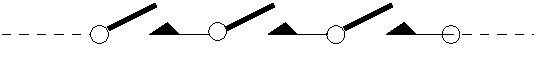
\includegraphics[width=4cm]{Figures/ET} \vspace{1cm}
\par\end{centering}
\caption{Fonction « ET » ~\textendash{} \textbf{produit} $a.b.c=Y$}

\label{fig:ET} 
\end{figure}


\subsection{Produel}

Il faut choisir un symbolisme simple qui puisse traduire dans l'expression
écrite, la dualité qui caractérise les ensembles binaires et qui permette,
en utilisant si possible les deux dimensions du plan, l'établissement
de relations duales élémentaires.

Nous savons aussi, par dualité, qu'il est possible de faire correspondre
au produit, la \textit{fonction algébrique binaire} :

\centerline{$\pi=1-P$} \centerline{$\pi=1-(1-f_{1}).(1-f_{2})\ldots(1-f_{n})=\overline{f_{1}.f_{2}\ldots f_{n}}$}
\centerline{$f_{i}\in E_{01},\forall i=1,2,\ldots n)\Longrightarrow(\pi\in E_{01})$}

La fonction $\pi$ est égale à zéro lorsque toutes les fonction $f_{i}$
sont simultanément nulles,

\centerline{$f_{1}=f_{2}=\ldots=f_{n}=0)\Longrightarrow(\pi=0)$}

et qu'elle est égale à l'unité dans tous les autres cas, puisqu'il
suffit qu'une fonction $f_{i}$ au moins soit égale à l'unité pour
que le produit algébrique $(1-f_{1}).(1-f_{2})\ldots(1-f_{n})$ soit
nul ; ce qui entraîne $\pi=1$.

Nous conviendrons alors de représenter la fonction « $\pi$ » ~,
que nous appellerons « \textit{produel} » ~\footnote{Les racines latines « pro » et « duales » ont été choisies
dans la constitution du né\-o\-lo\-gisme « pro\-duel » pour
marquer d'une part la nécessité de conserver la dualité dans les expressions
binaires et aussi par analogie avec le mot « produit » ~.} en groupant les termes qui la composent suivant une colonne verticale
par analogie avec l'écriture horizontale du produit, pour traduire
dans le symbolisme, la propriété de dualité.

\begin{center}
$\pi=\begin{array}{|c|}
f_{1}\\
f_{2}\\
\vdots\\
f_{n}
\end{array}=1-(1-f_{1}).(1-f_{2})\ldots(1-f_{n})=\overline{f_{1}.f_{2}\ldots F_{n}}$
\end{center}

Nous appellerons également « $\pi$ » ~, fonction « OU »  dans
le cas des applications technologiques.

\begin{figure}[htb]
\center{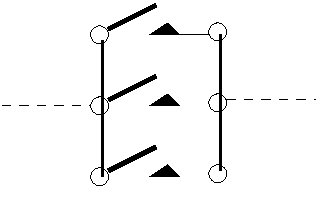
\includegraphics[width=4cm]{Figures/OU}} \vspace{1cm}

\setbox1=\hbox{$\begin{array}{r|c|l}
 & a\\
\text{Fonction «  OU » {\bf produel} : }  & b & =1-(1-a).(1-b).(1-c)=Z\\
 & c
\end{array}$} 

\caption{\box1}

\label{fig:OU} 
\end{figure}


\subsection{Définition d'une \emph{structure logique binaire}}

La structure logique binaire se caractérise essentiellement par les
deux opérations fondamentales qui ont des propriétés réciproques.
Les symboles peuvent représenter des ensembles, des partitions d'ensembles,
des groupes, des classes ou des éléments, voire même des opérateurs.

Les deux opérations sont, à la fois, \textbf{commutatives, associatives,
réciproquement distributives} et possèdent, toutes deux, \textbf{la
propriété d'idempotence} ; ce qui permet d'écrire successivement les
égalités suivantes~:

\begin{center}
{\scriptsize{}}%
\begin{tabular}{|l|l|}
\hline 
\multicolumn{1}{|c|}{\textit{\scriptsize{}Produit}} & \multicolumn{1}{|c|}{\textit{\scriptsize{}Produel}}\tabularnewline
\hline 
 & \tabularnewline
{\scriptsize{}$P=a.b.c$ } & {\scriptsize{}$\begin{array}{rcl}
\pi & = & \begin{array}{|c|}
a\\
b\\
c
\end{array}\\
 & = & 1-(1-a).(1-b).(1-c)
\end{array}$ }\tabularnewline
{\scriptsize{}\textendash{} élément neutre « 1 » ~} & {\scriptsize{}\textendash{} élément neutre « 0 » ~}\tabularnewline
\multicolumn{1}{|c|}{{\scriptsize{}$(1.f)=f$}} & \multicolumn{1}{|c|}{{\scriptsize{}$\begin{array}{|c|}
0\\
f
\end{array}=f$}}\tabularnewline
{\scriptsize{}\textendash{} élément absorbant « 0 » ~} & {\scriptsize{}\textendash{} élément absorbant « 1 » ~}\tabularnewline
\multicolumn{1}{|c|}{{\scriptsize{}$(0.f)=0$}} & \multicolumn{1}{|c|}{{\scriptsize{}$\begin{array}{|c|}
1\\
f
\end{array}=1$}}\tabularnewline
{\scriptsize{}\textendash{} commutatif : $\begin{array}{|c|}
ab\end{array}=\begin{array}{|c|}
ba\end{array}$ } & {\scriptsize{}\textendash{} commutatif : $\begin{array}{|c|}
a\\
b
\end{array}=\begin{array}{|c|}
b\\
a
\end{array}$ }\tabularnewline
{\scriptsize{}\textendash{} associatif : $\begin{array}{|c|c||}
a & bc\end{array}=\begin{array}{||c|c|}
ba & c\end{array}=\begin{array}{|c|}
cba\end{array}$ } & {\scriptsize{}\textendash{} associatif : $\begin{array}{||c||}
\multicolumn{1}{|c|}{a}\\
b\\
c
\end{array}=\begin{array}{||c||}
b\\
a\\
\multicolumn{1}{|c|}{c}
\end{array}=\begin{array}{|c|}
c\\
b\\
a
\end{array}$ }\tabularnewline
 & {\scriptsize{}\textendash distributif : }\tabularnewline
{\scriptsize{}\textendash{} distributif : $\begin{array}{|c|}
ab\\
ac\\
d
\end{array}=\begin{array}{|c|}
a\;\begin{array}{|c}
b\\
c
\end{array}\\
d
\end{array}=\begin{array}{|c|}
d\\
\begin{array}{c|}
b\\
c
\end{array}\;a
\end{array}=\begin{array}{|c|}
d\\
b\\
c
\end{array}\begin{array}{c|}
d\\
a
\end{array}$ } & {\scriptsize{}$\begin{array}{|c|c|}
a & a\\
b & c
\end{array}\begin{array}{c|}
d\end{array}=\begin{array}{|c|}
a\\
bc
\end{array}=\begin{array}{|c}
d\end{array}\begin{array}{|c|}
bc\\
a
\end{array}=\begin{array}{|c|}
dbc\\
da
\end{array}$}\tabularnewline
{\scriptsize{}\textendash{} idempotent : $\begin{array}{|c|}
aa\ldots a\end{array}=\begin{array}{|c|}
a\end{array}$ } & {\scriptsize{}\textendash{} idempotent : $\begin{array}{|c|}
a\\
a\\
\vdots\\
a
\end{array}=\begin{array}{|c|}
a\end{array}$ }\tabularnewline
\multicolumn{1}{|c|}{{\scriptsize{}$P=\overbrace{a.a\ldots a}^{n}=a^{n}$}} & \multicolumn{1}{|c|}{{\scriptsize{}$\pi=\left.\begin{array}{|c|}
a\\
a\\
\vdots\\
a
\end{array}\right\} n=1-(1-n)^{n}$}}\tabularnewline
\multicolumn{1}{|c|}{{\scriptsize{}pour $a=0\hfil(0)^{n}=0$}} & \multicolumn{1}{|c|}{{\scriptsize{}pour $a=0\hfil\pi=1-(1)^{n}=0$}}\tabularnewline
\multicolumn{1}{|c|}{{\scriptsize{}pour $a=1\hfil(1)^{n}=1$}} & \multicolumn{1}{|c|}{{\scriptsize{}pour $a=1\hfil\pi=1-(1)^{n}=1$}}\tabularnewline
\multicolumn{1}{|l|}{{\scriptsize{} }%
\begin{minipage}[t]{7.5cm}%
{\scriptsize{} Si dans un produit, deux facteurs sont complémentaires,
le produit est nul. }%
\end{minipage}} & \multicolumn{1}{|l|}{{\scriptsize{} }%
\begin{minipage}[t]{6cm}%
{\scriptsize{} Si dans un produel, deux facteurs duals sont complémentaires,
le produel est égal à l'unité }%
\end{minipage}}\tabularnewline
{\scriptsize{}$P=f.\overline{f}.P_{1}$ } & {\scriptsize{}$\pi=\begin{array}{|c|}
f\\
\overline{f}\\
\pi_{1}
\end{array}=1-(1-f).f.(1-\pi_{1})$ }\tabularnewline
{\scriptsize{}$P=f.(1-f)P_{1}=(f-f^{2}).P_{1}$ } & {\scriptsize{}$=1-(f-f^{2}).(1-\pi_{1}=1-0.(1-\pi_{1})$ }\tabularnewline
{\scriptsize{}$P=(0.P_{1})=0$ } & {\scriptsize{}$\pi=\begin{array}{|c|}
1\\
\pi_{1}
\end{array}=1$ }\tabularnewline
{\scriptsize{}$(f.\overline{f})=0$ } & {\scriptsize{}$\begin{array}{|c|}
f\\
\overline{f}
\end{array}=1$ }\tabularnewline
\hline 
\end{tabular} 
\end{center}

\subsection{Théorème de De Morgan}

Ce théorème est contenu implicitement dans les définitions précédentes.

\begin{center}
$1-\begin{array}{|c|}
f_{1}\\
f_{2}\\
\vdots\\
f_{n}
\end{array}=\overline{\begin{array}{|c|}
f_{1}\\
f_{2}\\
\vdots\\
f_{n}
\end{array}}=\overline{f_{1}}.\overline{f_{2}}\ldots\overline{f_{n}}=(1-f_{1}).(1-f_{2})\ldots(1-f_{n})$
\end{center}

\textit{Le complément d'un produel est égal au produit des compléments
des facteurs duals qui le composent.}

\begin{center}
$\overline{f_{1}.f_{2}\ldots f_{n}}s=\begin{array}{|c|}
\overline{f_{1}}\\
\overline{f_{2}}\\
\vdots\\
\overline{f_{1}}
\end{array}=1-(f_{1}.f_{2}\ldots f_{n})$
\end{center}

\textit{Le complément d'un produit est égal au produel des compléments
des facteurs qui le composent}.

\subsection{Fonctions canoniques et tables de vérité}

Toute fonction binaire peut s'exprimer soit par un produit de produels
soit par un produel de produits. Les expressions obtenues sont appelées
« \textit{fonctions canoniques} » ~.

Si une fonction binaire dépend de « $n$ » variables distinctes
$x_{1},x_{2},\ldots x_{n}$, nous ne pouvons envisager au total que
$2^{n}$ combinaisons de valeurs distinctes (0 ou 1) de ces « $n$ » variables.
Si la fonction binaire est égale à l'unité pour « $p$ »  combinaisons,
elle est nécessairement ????????????????

Nous appellerons « \textit{ transposition}  » \label{transposition}~,
\textit{le passage, pour une même fonction, de la première à la deuxième
forme canonique et réciproquement}.

\subsubsection{Établissement de la première forme canonique}

On inscrit horizontalement les variables dans un ordre quelconque,
puis on porte successivement sous ces variables dans le sens horizontal,
les combinaisons de valeurs pour lesquelles la fonction est égale
à l'unité. Il suffit alors de remplacer respectivement dans le tableau
obtenu, chaque valeur « 1 » ~par la variable « $x_{k}$ » ~de
la même colonne et chaque valeur « 0 » ~par le complément $\overline{x_{k}}$
de la variable de la même colonne.

\textit{Exemple :} 

Établir la première forme canonique d'une fonction de trois variables
$x_{1},x_{2},x_{3}$, égale à l'unité lorsqu'une des variables est
égale à l'unité, les deux autres étant nulles.

La table de vérité s'écrit :

\begin{center}
\begin{tabular}{|c|c|c||c|}
\hline 
$x_{1}$  & $x_{2}$  & $x_{3}$  & $f$ \tabularnewline
\hline 
1  & 0  & 0  & 1 \tabularnewline
0  & 1  & 0  & 1 \tabularnewline
0  & 0  & 1  & 1 \tabularnewline
\hline 
\end{tabular}
\end{center}

La première forme canonique s'établit immédiatement à partir de la
table de vérité :

\[
f=\begin{array}{|c|}
x_{1}.\overline{x}_{2}.\overline{x}_{3}\\
\overline{x}_{1}.x_{2}.\overline{x}_{3}\\
\overline{x}_{1}.\overline{x}_{2}.x_{3}
\end{array}
\]


\subsubsection{Établissement de la deuxième forme canonique}

Pour établir la deuxième forme canonique relative aux combinaisons
de valeurs de « \textit{n} » ~variables pour lesquelles cette fonction
est nulle, on inscrit verticalement les variables $x_{1},x_{2},\ldots,x_{n}$
dans un ordre quelconque et successivement dans le même ordre vertical,
les combinaisons de valeurs pour lesquelles $f=0$. Il suffit alors
d'écrire les produit des produels obtenus en remplaçant respectivement
dans ce tableau, chaque valeur « 0 » ~par la variable « $x_{k}$ » \-~de
la même ligne et chaque valeurs « 1 » \-~par le complément « $\overline{x}_{k}$ » \-~de
la variable de la même ligne.

\textit{Exemple :}

Établir la deuxième forme canonique d'une fonction de trois variables
$x_{1},x_{2},x_{3}$, égale à zéro lorsque deux au moins des trois
variables sont égales à l'unité.

La table de vérité s'écrit :

\begin{center}
\begin{tabular}{|c|c|c||c|}
\hline 
$x_{1}$  & $x_{2}$  & $x_{3}$  & $f$ \tabularnewline
\hline 
0  & 1  & 1  & 0 \tabularnewline
1  & 0  & 1  & 0 \tabularnewline
1  & 1  & 0  & 0 \tabularnewline
1  & 1  & 1  & 0 \tabularnewline
\hline 
\end{tabular}
\end{center}

Comme nous l'avons indiqué précédemment, nous en tirons le tableau
:

\[
\begin{array}{c|c|c|c|c|}
x_{1} & 0 & 1 & 1 & 1\\
x_{2} & 1 & 0 & 1 & 1\\
x_{3} & 1 & 1 & 0 & 1
\end{array}
\]

d'où la fonction cherchée :

\[
f=\begin{array}{|c|c|c|c|}
{x}_{1} & \overline{x}_{1} & \overline{x}_{1} & \overline{x}_{1}\\
\overline{x}_{2} & {x}_{2} & \overline{x}_{2} & \overline{x}_{2}\\
\overline{x}_{3} & \overline{x}_{3} & {x}_{3} & \overline{x}_{3}
\end{array}
\]


\subsection{Présentation des tables de vérité}

\subsubsection{Tables de vérité complète.}

\textendash{} Nous dirons qu'une table de vérité est complète lorsqu'elle
fait apparaître la totalité des « $2^{n}$ » \-~combinaisons de
valeurs possibles, relatives aux « \textit{n} » \-~variables dont
dépend la fonction.

Nous conviendrons d'inscrire les valeurs (0 ou 1) que prend la fonction
à droite d'un double trait vertical de séparation et sur la même ligne
que la combinaison correspondante des valeurs des variables.

Ainsi la table de vérité complète d'une fonction de trois variables,
$F(a,b,c)$, peut s'écrire par exemple :

\begin{center}
\begin{tabular}{r|c|c|c||c|}
\multicolumn{1}{c}{} & \multicolumn{4}{c}{\textit{Table de vérité}}\tabularnewline
\cline{2-5} 
 & a  & b  & c  & F \tabularnewline
\cline{2-5} 
0  & 0  & 0  & 0  & 1 \tabularnewline
1  & 0  & 0  & 1  & 0 \tabularnewline
2  & 0  & 1  & 0  & 0 \tabularnewline
3  & 0  & 1  & 1  & 0 \tabularnewline
4  & 1  & 0  & 0  & 1 \tabularnewline
5  & 1  & 0  & 1  & 0 \tabularnewline
6  & 1  & 1  & 0  & 1 \tabularnewline
7  & 1  & 1  & 1  & 1 \tabularnewline
\cline{2-5} 
\end{tabular}\medskip
\end{center}

Il est souvent intéressant de faire figurer dans une colonne, à gauche,
des repères décimaux qui correspondent aux nombres représentés par
les chiffres binaires $a,b,c$, en plaçant ces nombres dans l'ordre
naturel. Cette disposition permet, en particulier, de s'assurer qu'aucune
combinaison n'a été oubliée.

Une table de vérité complète autorise, en suivant les règles énoncées
précédemment, \emph{l'écriture immédiate de la fonction sous deux
formes canoniques}. 

En ce qui concerne l'exemple donné nous pouvons écrire :

\begin{center}
F $=$ %
\begin{tabular}{|c|}
$\begin{array}{ccc}
\bar{a} & \bar{b} & \bar{c}\\
a & \bar{b} & \bar{c}\\
a & b & \bar{c}\\
a & b & c
\end{array}$\tabularnewline
\end{tabular}= %
\begin{tabular}{|c|c|c|c|}
$\begin{array}{c}
a\\
b\\
\bar{c}
\end{array}$ & $\begin{array}{c}
a\\
\bar{b}\\
c
\end{array}$ & $\begin{array}{c}
a\\
\bar{b}\\
\bar{c}
\end{array}$ & $\begin{array}{c}
\bar{a}\\
b\\
\bar{c}
\end{array}$\tabularnewline
\end{tabular}
\end{center}

La première forme utilise les combinaisons pour lesquelles F $=1,(0,4,6,7)$et
la seconde forme les combinaisons pour lesquelles F $=0,(1,2,3,5)$.

\subsubsection{Tables de vérité incomplète. }

\textendash{} Une fonction binaire est entièrement définie si l'on
connaît seulement les combinaisons des valeurs pour lesquelles elle
conserve la même valeur (0 ou 1).

Nous appellerons, par définition, table de vérité incomplète, le tableau
dans lequel sont inscrite ces combinaisons. Nous préciserons à droite
de ce tableau, la valeur correspondante de la fonction. Pour chaque
fonction i l existe  donc deux tables de vérité incomplètes.

Les deux tables de vérité incomplètes qui correspondent à la fonction
précédente F $(a,b,c)$ peuvent s'écrire suivant que l'on choisit
pour \og F \fg{} la valeur \og 0 \fg{} ou la valeur \og 1 \fg{}
: 

% \hspace*{1cm}%
\bigskip 

\begin{tabular}{c|c|c|c||c|}
\multicolumn{1}{c}{} & \multicolumn{4}{c}{\emph{Table de vérité }(F = 1)}\tabularnewline
\cline{2-5} 
 & $a$ & $b$ & $c$ & F\tabularnewline
\cline{2-5} 
0 & 0 & 0 & 0 & \tabularnewline
4 & 1 & 0 & 0 & \tabularnewline
6 & 1 & 1 & 0 & F = 1\tabularnewline
7 & 1 & 1 & 1 & \tabularnewline
\cline{2-5} 
\end{tabular}\hspace*{\fill}%
\begin{tabular}{c|c|c|c||c|}
\multicolumn{1}{c}{} & \multicolumn{4}{c}{\emph{Table de vérité }(F = 0)}\tabularnewline
\cline{2-5} 
 & $a$ & $b$ & $c$ & F\tabularnewline
\cline{2-5} 
1 & 0 & 0 & 1 & \tabularnewline
2 & 0 & 1 & 0 & \tabularnewline
3 & 0 & 1 & 1 & F = 0\tabularnewline
5 & 1 & 0 & 1 & \tabularnewline
\cline{2-5} 
\end{tabular}\hspace*{1cm}

\bigskip{}

Une table de vérité incomplète ne permet d'écrire que l'une des deux
formes canoniques. La propriété de dualité la rend cependant suffisante
pour définir complètement une fonction binaire.

\subsubsection{Tables de vérité réduite.}

\textendash{} Ce sont des tables de vérité incomplètes dans lesquelles
certaines combinaisons sont regroupées afin de tenir compte d'une
partie ou de la totalité \emph{des adjacences} qui existent entre
elles. Ces adjacences étant repérées dans la tables par le symbole
\og $\phi$ \fg{} qui signifie que la valeur prise par la variable
peut être indifféremment \og 0 \fg{} ou \og 1 \fg{}. Nous pouvons
tirer de l'exemple précédent différentes tables de vérité réduites,
parmi lesquelles les deux suivantes : 

\bigskip{}

\hspace*{1cm}%
\begin{tabular}{c|c|c|c||c|}
\cline{2-5} 
 & $a$ & $b$ & $c$ & F\tabularnewline
\cline{2-5} 
0-4 & $\phi$ & 0 & 0 & $1$\tabularnewline
6-7 & 1 & 1 & $\phi$ & 1\tabularnewline
\cline{2-5} 
\end{tabular}\hspace*{\fill}%
\begin{tabular}{c|c|c|c||c|}
\cline{2-5} 
 & $a$ & $b$ & $c$ & F\tabularnewline
\cline{2-5} 
1-5 & $\phi$ & 0 & 1 & 0\tabularnewline
2-3 & 0 & 1 & $\phi$ & 0\tabularnewline
\cline{2-5} 
\end{tabular}\hspace*{1cm}

\bigskip{}

l'adjacence, comme nous le verrons quand nous étudierons les simplifications,
a pour effet de supprimer la variable biforme (directe et complémentée)
dans le produit ou le produel qui résulte des combinaisons groupées.
Une table de vérité réduite ne donne donc plus une forme canonique
mais une forme déjà simplifiée. Dans le cas envisagé, nous tirons
de la première table de vérité réduite :

\bigskip{}

\begin{center}
F = %
\begin{tabular}{|c|}
$\begin{array}{ccc}
\bar{b} & . & \bar{c}\\
a & . & b
\end{array}$\tabularnewline
\end{tabular}
\end{center}

\bigskip{}

de la seconde table de vérité réduite nous tirons :

\begin{center}
F = %
\begin{tabular}{|c|c|}
$\begin{array}{c}
b\\
\bar{c}
\end{array}$ & $\begin{array}{c}
\end{array}$$\begin{array}{c}
a\\
\bar{b}
\end{array}$\tabularnewline
\end{tabular}
\end{center}

\subsection{Transformations des formes canoniques}

Nous allons examiner maintenant quelques transformations simples que
peuvent subir les formes canoniques compte tenu des théorèmes déjà
établis.

\subsubsection{Transpositions.}

\textendash{} Nous avons appelé (page\pageref{transposition}\emph{)
transposition, le passage, pour une même fonction, de la première
à la deuxième forme canonique ou réciproquement.}

Pour transposer une fonction de \og n \fg{} variables, mise sous
forme canonique, il est recommandé d'écrire pour cette fonction, une
table de vérité complète en inscrivant les \og $2^{n}$ \fg{} combinaisons
de valeurs des variables dans un ordre binaire naturel.

Si une fonction binaire de \og $n$ \fg{} variables, mise sous la
première forme canonique contient \og $p$ \fg{} produits, elle
contient nécessairement lorsqu'elle est transposée, \og $q$ \fg{}
produels tels que $p+q=2$$^{n}$.

il en résulte que la transposition est un moyen de simplification
dans le cas où le nombre de produits ou de produels d'une fonction
canonique de \og $n$ \fg{} variables est supérieur à \og $2^{n-1}$ \fg{}.

\subsubsection{Complémentations }

\textendash{} L'application du théorème de De Morgan permet d'écrire
immédiatement la fonction complément d'une fonction canonique. Il
suffit de remplacer chaque produel par un produit et réciproquement,
en complémentant chacune des variables. Les lignes horizontales deviennent
des colonnes verticales, les colonnes deviennent des lignes horizontales
et les variables se trouvent complémentées. La simplicité de la compréhension
résulte de l'aspect dual du symbolisme adopté. 

A titre d'exemple, la fonction 

\medskip

\begin{center}
$f=\left|\begin{array}{ccc}
\begin{array}{c}
x_{1}\\
\bar{x}_{2}\\
\bar{x}_{3}
\end{array} & \left|\begin{array}{c}
\bar{x}_{1}\\
x_{2}\\
\bar{x}_{3}
\end{array}\right| & \begin{array}{c}
\bar{x}_{1}\\
\bar{x}_{2}\\
x_{3}
\end{array}\end{array}\right|$
\end{center}

\medskip

peut être complémentée facilement, selon la méthode indiquée, et nous
obtenons :

\medskip

\begin{center}
$f=\left|\begin{array}{c}
\bar{x}_{1}.x_{2}.x_{3}\\
x_{1}.\bar{x}_{2}.x_{3}\\
x_{1}.x_{2}.\bar{x}_{3}
\end{array}\right|$
\end{center}

\medskip

\begin{flushleft}
Si la fonction ne se présente pas sous une forme canonique, la méthode
ce complémentation est identique et reste simple dans son application~;
ce qu'illustre les deux exemples suivants~:\medskip
\par\end{flushleft}

\begin{flushleft}
\medskip
\par\end{flushleft}

\hspace*{\fill}$f_{1}=\begin{array}{cc}
a & \left|\begin{array}{c}
b\\
\bar{c}.d
\end{array}\right|\end{array}$\hspace*{\fill}$\bar{f_{1}}=\left|\begin{array}{c}
\bar{a}\\
\begin{array}{cc}
\bar{b} & \left|\begin{array}{c}
c\\
\bar{d}
\end{array}\right.\end{array}
\end{array}\right|$\hspace*{\fill}

\medskip

\hspace*{\fill}$f_{2}=\left|\begin{array}{c}
\begin{array}{cc}
\bar{x_{1}} & \left|\begin{array}{c}
x\bar{x}\\
x_{3}
\end{array}\right.\end{array}\\
x_{2}.x_{3}
\end{array}\right|$\hspace*{\fill}$\bar{f_{2}}=\left|\begin{array}{cc}
\begin{array}{c}
\bar{x_{2}}\\
\bar{x_{3}}
\end{array} & \left|\begin{array}{c}
x_{1}\\
x_{2}.\bar{x_{3}}
\end{array}\right.\end{array}\right|$\hspace*{\fill}

\ifdefined\COMPLETE
\else
    \end{document}
\fi


\ifdefined\COMPLETE
\else
    \input{./preambule_Analyse_binaire.ltx}
    \begin{document}
\fi


\chapter{Simplification des fonctions binaires}

Par simplification des fonctions binaires, nous entendrons la réduction
du nombre des éléments littéraux~; c'est à dire la simplification,
en dehors de toute considération technologique, des expressions symboliques
écrites.

Le but poursuivi sera donc en général, la recherche et l'élimination
des termes \emph{redondants} : en définissant comme tel tout terme
qui peut être supprimé dans une fonction binaire sans apporter de
modification numérique relativement aux combinaisons de valeurs des
variables indépendantes.

Les simplifications devront être les conséquences démontrables des
propriétés algébriques des produits et des produels. Parmi les méthodes
essentielles nous étudierons en particulier les simplifications par
\emph{mise en facteur et développement, }par\emph{ adjacences, }par\emph{
transposition }et par\emph{ consensus} qui sont des méthodes fondamentales
et simples et s'avèrent suffisantes dans la plupart des cas.

\section{Mise en facteur et développements}

L'ensemble binaire \og E$_{10}$ \fg{} définit un anneau commutatif
automorphe, puisque \og E$_{10}=$ E$_{10}$ \fg{} et que l'on a
choisi deux lois algébriques internes de composition qui sont le produit
\og P $=x\cdot y$  \fg{}, et le produel : 

\medskip

$\pi=1-\left(1-x\right)\cdot\left(1-y\right)=\left|\begin{array}{c}
x\\
y
\end{array}\right|$.

\medskip

Il est intéressant de démontrer la propriété algébrique de distributivité
du produel par rapport au produit et réciproquement, du produit par
rapoort au produel. \textit{Cette réciprocité, qui résulte de la propriété
fondamentale de dualité, est une caractéristique essentielle et particulièrement
interessante des ensembles binaires.}

\subsection{Mise en facteur dans un produel. }

Considérons le produel :

\medskip

F$=\left|\begin{array}{ccc}
\varphi & \cdot & f_{1}\\
\varphi & \cdot & f_{2}
\end{array}\right|=1-\left(1-\varphi\cdot f_{1}\right)\cdot\left(1-\varphi\cdot f_{2}\right)$.

\medskip

L'expression algébrique développée s'écrit :

\medskip

F =$\varphi\cdot f_{1}+\varphi\cdot f_{2}-\varphi^{2}\cdot f_{1}\cdot f_{2}$,
en utilisant le théorème d'idempotence $\varphi^{2}=\varphi$, \\
F = $\varphi\cdot f_{1}+\varphi\cdot f_{2}-\varphi\cdot f_{1}\cdot f_{2}$,
que nous pouvons écrire :

\medskip

F$=1-\left(1-\varphi\cdot f_{1}\right)\cdot\left(1-\varphi\cdot f_{2}\right)=\varphi\cdot\left|\begin{array}{c}
f_{1}\\
f_{2}
\end{array}\right|$.

\medskip

Ainsi se trouve démontrée l'identité réciproque :

\medskip

\begin{center}
\fbox{\parbox[c]{0.3\textwidth}{%
\begin{center}
$\left|\begin{array}{ccc}
\varphi & \cdot & f_{1}\\
\varphi & \cdot & f_{2}
\end{array}\right|\equiv\varphi\cdot\left|\begin{array}{c}
f_{1}\\
f_{2}
\end{array}\right|$
\end{center}%
}}
\end{center}

\medskip

Nous appellerons \og mise en facteur~ \fg{} le passage de la première
expression à la seconde et \og développement \fg{} ou \og produits
effectués \fg{} le passage inverse.

L'identité précèdente peut être étendue à un produel contenant un
nombre quelconque de produits admettant \og  $\varphi$ \fg{} comme
facteur commun.

\medskip

Soit en effet la fonction F $=\left|\begin{array}{l}
P_{1}\\
P_{2}\\
\cdot\\
\cdot\\
\cdot\\
P_{q}\\
P_{q+1}\\
\cdot\\
\cdot\\
\cdot\\
P_{n}
\end{array}\right|$,

\medskip

dans laquelle, $P_{1=\varphi}\cdot f_{1}$, $P_{2=\varphi}\cdot f_{2}$,
\dots , $P_{q=\varphi}\cdot f_{q}$, $q\leq n$. Appellons $P_{12}^{'}=\varphi\cdot\left|\begin{array}{c}
f_{1}\\
f_{2}
\end{array}\right|$, la fonction obtenue en mettant \og $\varphi$ \fg{} en facteur
dans les deux premiers produits $P_{1}$ et $P_{2}$.

En groupant \og  $P_{12}^{'}$ \fg{} et \og $P_{3}$ \fg{}, nous
pouvons à nouveau mettre \og $\varphi$ \fg{} en facteur et nous
obtenons $P_{123}^{'}=\varphi\cdot\left|\begin{array}{c}
f_{1}\\
f_{2}\\
f_{3}
\end{array}\right|$, et ainsi de suite jusqu'à \og $P_{q}$ \fg{}. Ce qui permet d'écrire
l'identité :

\begin{center}
\medskip
\fbox{\parbox[c]{0.35\textwidth}{%
\begin{center}
$\left|\begin{array}{ccc}
\varphi & \cdot & f_{1}\\
\varphi & \cdot & f_{2}\\
 & .\\
 & .\\
 & .\\
\varphi & \cdot & f_{q}\\
 &  & P_{q+1}\\
 & .\\
 & .\\
 & .\\
 &  & P_{n}
\end{array}\right|\equiv\left|\begin{array}{l}
\varphi\cdot\left|\begin{array}{c}
f_{1}\\
f_{2}\\
.\\
.\\
.\\
f_{q}
\end{array}\right|\\
\begin{array}{l}
P_{q+1}\\
.\\
.\\
.\\
P_{n}
\end{array}
\end{array}\right|$
\end{center}%
}}
\end{center}

\medskip

Ainsi se trouyve démontrée la \emph{distributivité du produit par
rapport au produel}.

\subsection{Mise en «  facteur dual »  dans un produit}

Considérons la fonction : F $=\left|\begin{array}{l}
\varphi\\
f_{1}
\end{array}\right|\left.\begin{array}{l}
\varphi\\
f_{2}
\end{array}\right|$\medskip

Le développement algébrique de \og F \fg{} s'écrit :\medskip

$\begin{array}{rl}
\textrm{F} & =\left[1-\left(1-\varphi\right).\left(1-f_{1}\right)\right].\left[1-1\left(1-\varphi\right).\left(1-f_{2}\right)\right]\\
 & =1-\left(1-\varphi\right).\left(1-f_{1}\right)-\left(1-\varphi\right).\left(1-f_{2}\right)+\left(1-\varphi\right)^{2}.\left(1-f_{1}\right).\left(1-f_{2}\right)
\end{array}$\medskip

Le théorème d'idempotence permet d'écrire$\left(1-\varphi\right)^{2}=\left(1-\varphi\right)$,
d'où l'expression de \og F \fg{} :\medskip

$\begin{array}{rl}
\textrm{F} & =1-\left(1-\varphi\right).\left(1-f_{1}\right)-\left(1-\varphi\right).\left(1-f_{2}\right)+\left(1-\varphi\right).\left(1-f_{1}\right).\left(1-f_{2}\right)\\
 & =1-\left(1-\varphi\right).\left(1-f_{1}.f_{2}\right)=\left|\begin{array}{c}
\varphi\\
f_{1}.\,f_{2}
\end{array}\right|
\end{array}$

Nous avons ainsi démontré l'identité réciproque :\medskip

\begin{center}
\fbox{\parbox[c]{0.3\textwidth}{%
\begin{center}
$\left|\begin{array}{cc}
\begin{array}{c}
\varphi\\
f_{1}
\end{array} & \left|\begin{array}{c}
\varphi\\
f_{2}
\end{array}\right.\end{array}\right|\equiv\left|\begin{array}{c}
\varphi\\
f_{1}.\,f_{2}
\end{array}\right|$
\end{center}%
}}
\end{center}

Nous appellerons \og \emph{mise en facteur dual} \fg{}, le passage
de la première expression à la seconde et \og \emph{produels effectués} \fg{}
ou \og \emph{développement dual} \fg{} le passage inverse.

Comme pour le produel, l'identité précédente peut être étendue à
un produit contenant un nombre quelconque de produels admettant \og $\varphi$ \fg{}
commer \og facteur dual \fg{} commun.

soit :

\begin{center}
$\pi=\pi_{1}.\pi_{2}\text{\dots}\pi_{q}.\pi_{q+1}\text{\dots}\pi_{n}$
\end{center}

avec $\pi_{1=}\left|\begin{array}{c}
\varphi\\
f_{1}
\end{array}\right|$, $\pi_{2=}\left|\begin{array}{c}
\varphi\\
f_{2}
\end{array}\right|$, $\ldots\:\pi_{q=}\left|\begin{array}{c}
\varphi\\
f_{q}
\end{array}\right|$, $q\leq n$

nous pouvons de proche en proche mettre \og $\varphi$ \fg{} en
facteur dual dans les produels $\pi.\pi_{2}\text{\dots}\pi_{q}$,
et obtenir finalement l'identité \medskip

\begin{center}
\fbox{\parbox[c]{0.65\textwidth}{%
\begin{center}
$\left|\begin{array}{cccc}
\begin{array}{c}
\varphi\\
f_{1}
\end{array} & \left|\begin{array}{c}
\varphi\\
f_{2}
\end{array}\right| & \ldots & \left|\begin{array}{c}
\varphi\\
f_{q}
\end{array}\right.\end{array}\right|.\pi_{q+1}\ldots\pi_{n}\equiv\left|\begin{array}{c}
\varphi\\
f_{1}.\,f_{2}\ldots f_{q}
\end{array}\right|.\pi_{q+1}\ldots\pi_{n}$
\end{center}%
}}
\end{center}

Nous avons ainsi démontré \textsl{la distributivité du produel par
rapport au produit.} 

\newpage 

\section{Simplification élémentaires des fonctions binaires}

La propriété réciproque de distributivité des produits et produels
va nous permettre de tirer un certain nombre de conséquences et de
théorèmes élémentaires relatifs à la simplification des fonctions
binaires.

\subsection{Simplifications par développements. }

Si la mise en facteur fournit en général une forme simplifiées des
fonctions bianires, l'opération inverse par développement peut, dans
les cas que nous allons envisager, fournir également des simplifications
intéressantes. 

$1^{er}$ cas

\begin{center}
$\varphi.\left|\begin{array}{c}
f\\
A.\,\bar{\varphi}
\end{array}\right|=\left|\begin{array}{c}
\varphi.\,f\\
A.\,\varphi\,\bar{\varphi}
\end{array}\right|=\varphi.\,f$
\end{center}

Dans le cas particulier, souvent rencontré où $A=1$, nous pouvons
écrire : 

\begin{center}
$\varphi.\left|\begin{array}{c}
f\\
\bar{\varphi}
\end{array}\right|=\varphi.\,f$
\end{center}

$2^{e}$ cas

\begin{center}
$\left|\begin{array}{c}
\varphi\\
\begin{array}{cc}
f & \left|\begin{array}{c}
B\\
\bar{\varphi}
\end{array}\right.\end{array}
\end{array}\right|=\left|\begin{array}{cc}
\begin{array}{c}
\varphi\\
f
\end{array} & \left|\begin{array}{c}
\varphi\\
\overline{\varphi}\\
B
\end{array}\right|\end{array}\right.=\left|\begin{array}{c}
\varphi\\
f
\end{array}\right|$

\end{center}

Dans le cas particulier, souvent rencontré où $B=0$, nous pouvons
écrire : 

\begin{center}
$\left|\begin{array}{c}
\varphi\\
\begin{array}{cc}
f & .\end{array}\overline{\varphi}
\end{array}\right|=\left|\begin{array}{c}
\varphi\\
f
\end{array}\right|$
\end{center}

\subsection{Implications. }

Nous savons que la condition nécessaire et suffisante pour qu'un produit
binaire soit égal à l'unité, est que chacun des facteurs soit égal
à l'unité.

\begin{center}
$(P=f_{1}.f_{2}.\ldots f_{n}.=1)\Longleftrightarrow f_{1}=f_{2}=\ldots=f_{n}=1$
\end{center}

Nous pouvons donc appeler chaque facteur$f_{1},f_{2},\ldots f_{n},$
\textsl{implicant direct}, ou \textsl{implicant }de l fonction \og P \fg{}.

\begin{itemize}
\item \textsl{Toute fonction partielle pouvant être mise en facteurs dans une fonction donnée, sera donc un implicant de cette dernière.}

Nous savons également que la condition nécessaire et suffisante pour qu'un produel soit nul, est que chaque facteur dual soit égal à zéro.

\medskip 

$ \left( \pi = \left| \begin{array}{c} 
                f_1 \\ f_2 \\ . \\ . \\ . \\ f_n\\
                          \end{array}
                    \right| = 0 
  \right) \Longleftrightarrow (f_1 = f_2 = \ldots = f_n = 0 )  
$ 

\item \textsl {Toute fonction partielle pouvant être mise en facteur dual dans une fonction donnée sera,  par définition, un implicant dual de cette dernière.
}

\item Considérons le produit ayant pour facteurs un produel et l'un de ses implicants duals . F = $\varphi . \begin{vmatrix} \varphi \\ f \\ \end{vmatrix} $. « $0$ » étant l'élément neutre du produel, nous pouvons écrire : 

\centerline { $\varphi = \begin{vmatrix} \varphi \\ 0 \\ \end{vmatrix} \qquad \text{ et }  \qquad 
F =  \left| \begin{array}{c|c} \varphi & \varphi \\ 0 & f \\
\end{array} \right|$   
} 

En mettant « $\varphi$ » en facteur dual nous obtenons : 

\centerline{
$F = \begin{vmatrix} \varphi \\ 0 . f \\ \end{vmatrix} = \varphi $ 
}

De même le produel ayant pour facteurs duals un produit et l'un de ses implicants, s'écrit : 

\centerline  {
$ F' = \begin{vmatrix} \varphi \\  \varphi . f \\ \end{vmatrix} = \begin{vmatrix} \varphi .1 \\ \varphi  . f \\ \end{vmatrix} = \varphi . \begin{vmatrix} 1  \\  f \\ \end{vmatrix} = \varphi $   
} 

\end{itemize}

Nous tirons de ces égalité les deux théorèmes suivants : 

\subsection{Théorèmes. } \textsl{
Le produit d'une fonction binaire et de l'un quelconque de ses implicants duals, est égal à cet implicant dual. } 

\centerline{ \fbox{  $  \varphi \begin{vmatrix} \varphi \\  f \\ \end{vmatrix} = \varphi $} } 

Le produel d'une fonction binaire et de l'un quelconque de ses implicants directs, est égal à cet implicant dual.  

\centerline{ \fbox{  $  \varphi \begin{vmatrix} \varphi \\  \varphi . f \\ \end{vmatrix} = \varphi $} } 

\subsection{Adjacences. } \textsl{ Deux produits « $P_1$ » et « $P_2$ » sont dits adjacents lorsque l'on peut passer de l'un à l'autre en complémentant l'un des facteurs et ce facteur seulement. }

\bigskip 




Nous pouvons également par dualité définir l'adjacence pour deux produels. 

\textsl{Deux produels « ${\pi}_1$ »  et  « ${\pi}_2$ »  sont dits adjacents lorsque l'on peut passer de l'un à l'autre en complémentant l'un des facteurs duals et ce facteur seulement.  } 

\bigskip 

\centerline{ ${\pi}_1  = \begin{vmatrix} \varphi \\  f \\ \end{vmatrix} \qquad 
                                        {\pi}_2 = \begin{vmatrix} \overline{\varphi}  \\  f \\ \end{vmatrix}  $ }
                    
\subsection{Théorèmes. } \textsl{ Le produel de deux produits adjacents est égal au facteur commun aux deux produels}. 

\bigskip 

\centerline{ $ \begin{vmatrix}
P_1\\P_2\\
\end{vmatrix} 
 = \begin{vmatrix}
        \varphi . f \\ \overline{\varphi} . f \\
    \end{vmatrix} 
       = \begin{vmatrix}
            \varphi \\ \overline{\varphi} \\ 
        \end{vmatrix} .f = f 
  $ }

\bigskip 

 \textsl{ Le produel de deux produels adjacents est égal au facteur dual commun  aux deux produels}. 
 
 \bigskip 
 
 \centerline{$
 {\pi}_1 . {\pi}_2 = \left| \begin{array}{c|c} 
                                    \varphi & \overline{\varphi}  \\
                                    f & f \\
                       \end{array}  \right|
       = \begin{vmatrix}
               \varphi . \overline{\varphi} \\ f   \\
       \end{vmatrix} = f 
 $}
 
 \bigskip 

La fonction « $\varphi$ » est appelée « \textsl {fonction adjacente} » ou « \textsl {variable adjacente}  » lorsqu'il s'agit d'une simple variable.   

\newpage 

\section{Méthodes générales de simplification utilisant la mise en facteur} 

Considérons le produit de produels suivant 


\bigskip 

\centerline{ $
F_1 = \left|\begin{array}{c} 
            f_1 \\ f_3 \\
        \end{array}\right. 
        \left|\begin{array}{c} 
            f_1 \\ f_4 \\ f_7 \\
        \end{array}\right. 
         \left|\begin{array}{c} 
            f_1 \\ f_5 \\ f_6 \\ f_7 
        \end{array}\right| 
$ }

\bigskip 

« $F_1$ » peut s'écrire après mise en facteur dual de « $f_1$ » puis de « $f_7$ » :

\bigskip 

\centerline{
\begin{tikzpicture} [scale=.75]
%  \draw[help lines] (-2,-1) grid (15,6);
  \SetGraphUnit{1}    \GraphInit[vstyle=Empty]
\node [VertexStyle] (A) at (-1, 2) {$F_1 = \quad $} ;  
\node [VertexStyle] (a) at (3,4) {$f_1$} ;  
\node [VertexStyle] (c) at (1,1.5) {$f_3$} ;  
\node [VertexStyle] (d) at (3,2.5) {$f_4$} ;  
\node [VertexStyle] (e) at (5,3) {$f_5$} ;  
\node [VertexStyle] (f) at (5,2) {$f_6$} ;  
\node [VertexStyle] (g) at (3,1) {$f_7$} ;  
\draw [thick] (-.5,2) -- (0,2) ; 
\draw [thick] (2,1.5) -- (c)  -- (0,1.5) -- (0,4) -- (a) ; 
\draw [thick] (d) -- (2,2.5) -- (2,1) --  (g) ; 
\draw [thick] (a) -- (6,4) -- (6,1) -- (g) ; 
\draw [thick] (d) -- (4,2.5)  ;
\draw [thick] (f) -- (4,2) -- (4,3) -- (e) ; 
\draw [thick] (e) -- (6,3)  ;
\draw [thick] (f) -- (6,2)  ;
%
\node [VertexStyle] (B) at (6.75, 2.5) {$\;  =\; $} ;  
\node [VertexStyle] (s) at (9.2,4) {$f_7$} ;  
\node [VertexStyle] (m) at (9.2,1) {$f_1$} ;  
\node [VertexStyle] (n) at (12,2.4) {$f_3$} ;  
\node [VertexStyle] (p) at (8,2.5) {$f_4$} ;  
\node [VertexStyle] (q) at (9.75,2) {$f_5$} ;  
\node [VertexStyle] (r) at (9.75,3) {$f_6$} ;  
\draw [thick] (6,2.5) -- (B) -- (7.5,2.5) -- (7.5,1) -- (7.5,4)  -- (s)  -- (11, 4) -- (11,2) -- (q)  ; 
\draw [thick] (7.5,1) -- (m)  ; 
\draw [thick] (p) -- (8.9, 2.5)    ; 
\draw [thick] (q) -- (8.9, 2) -- (8.9, 3) -- (r)  -- (11, 3) ; 
\draw [thick] (11,2.4) -- (n) -- (13, 2.4)  ; 
\draw [thick] (12.4, 2.4) --  (12.4,1) -- (m)     ; 
\end{tikzpicture}
}

Lorsque les fonctions ne remplissent pas complètement l'espace qu'elles occupent entre les deux traits verticaux qui symbolisent les produels, on peut compléter par des traits continus horizontaux comme cela est indiqué dans les expression simplifiées de la fonction « $F_1$ » ci-dessus.

\begin{itemize}
\item Considérons d'autre part le produel de produits : 

\bigskip 

\centerline{ $ F_2 = \begin{vmatrix}
f_1 . f_4 . f_7 \\
f_1 . f_5 . f_6 . f_7\\
f_1 . f_3 \\
\end{vmatrix}$ }

\bigskip 

En mettant successivement « $f_7$ » et « $f_1$ » en facteur, nous obtenons : 

\bigskip 

\centerline{
\begin{tikzpicture} [scale=.75]
% \draw[help lines, color=red!25] (-2,-1) grid (15,5);
  \SetGraphUnit{1}    \GraphInit[vstyle=Empty]
\node [VertexStyle] (A) at (-.3, 2) {$F_2 = $} ;  
\node [VertexStyle] (a) at (1,2) {$f_1$} ;  
\node [VertexStyle] (c) at (4,1) {$f_3$} ;  
\node [VertexStyle] (d) at (5,3.5) {$f_4$} ;  
\node [VertexStyle] (e) at (5,2.5) {$f_5.f_6$} ;  
\node [VertexStyle] (f) at (3,3) {$f_7$} ;  
\node [VertexStyle] (B) at (6.5, 2) {$ = $} ;  
\draw [thick] (A) -- (a) -- (1.75,2) -- (1.75, 1) -- (c)  ; 
\draw [thick] (1.75,2) -- (1.75, 3) -- (f) -- (4, 3) -- (4,3.5) -- (d)  -- (6,3.5) -- (6, 1) -- (c) ; 
\draw [thick] (4, 3) -- (4,2.5)  -- (e) -- (6, 2.5) ; 
\draw [thick] (6, 2) --  (B)  ; 
%
\node [VertexStyle] (s) at (9.2,3.5) {$f_3$} ;  
\node [VertexStyle] (m) at (10,2.5) {$f_5.f_6$} ;  
\node [VertexStyle] (n) at (12.5,2) {$f_1$} ;  
\node [VertexStyle] (p) at (10,1) {$f_4$} ;  
\node [VertexStyle] (q) at (8.25,1.75) {$f_7$} ;  
\draw [thick]   (B)  -- (7.25, 2) -- (7.25, 1.75) -- (q) -- (9, 1.75)  -- (9,1) -- (p)  ; 
\draw [thick]   (9, 1.75)  -- (9,2.5) -- (m)  -- (11.5, 2.5)  -- (11.5, 2) -- (n) -- (13.5, 2) ; 
\draw [thick]   (7.25, 2) -- (7.25, 3.5) -- (s)  --(11.5, 3.5) -- (11.5, 1) -- (p)    ; 
\end{tikzpicture}
}

\item Les produits et les produels sont commutatifs, les colonnes ou les lignes des fonctions binaires peuvent être permutées entre elles et par suite les mises en facteurs peuvent s'effectuer aussi bien en partant de la droite qu'en partant de la gauche pour un produit, et les mises en facteurs dual, en partant du haut ou en partant du bas pour un produel. 

\medskip 

Ces mises en facteurs peuvent même se faire simultanément à droite et à gauche pour la première forme (produit), ou en haut et en bas pour la deuxièmes forme (produel). \textsl{Cette façon de procéder introduit une solution étrangère}. 

\medskip 

\centerline{\fbox {\parbox [t]  {.7 \linewidth} { Il y a donc lieu de s'assurer que la solution étrangère introduite dans la simplification obtenue correspond à un produit nul.}} }

\newpage

Considérons en effet la fonction 

\setbox1= \hbox { $ F = \begin{vmatrix}
f_1 . f_5 \\
f_2 . f_3 . f_5 \\
f_2 . f_4 \\
\end{vmatrix} = $  }


\centerline{\begin{tikzpicture} [scale=.75]
%  \draw[help lines, color=red!25] (-4,0) grid (7,5);
\SetGraphUnit{1}    \GraphInit[vstyle=Empty]    
\node [VertexStyle] (A) at (-1.75, 2) {\box1} ;  
% \node  (O) at (0,0) {$\times$} ;  
\node [VertexStyle] (a) at (1.75,1) {$f_2$} ;  
\node [VertexStyle] (b) at (3,3) {$f_1. f_5$} ;  
\node [VertexStyle] (c) at (4,1.5) {$f_3. f_5$} ;  
\node [VertexStyle] (d) at (4,0.5) {$f_4$} ;  
\draw [thick] (A) -- (1,2) -- (1,1) -- (a)  ; 
\draw [thick] (1,2) -- (1,3) -- (b)  -- (5,3) -- (5,.5) -- (d) -- (3,.5) -- (3, 1.5) -- (c)  ; 
\draw [thick]  (a) -- (3, 1) ; 
\draw [thick]  (c) -- (5.5, 1.5) ;  
\end{tikzpicture}
} 

\setbox1=\hbox{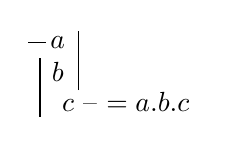
\begin{tikzpicture} [scale=.75]
%\draw[help lines, color=red!25] (-1,-1) grid (4,2);
\SetGraphUnit{1}    \GraphInit[vstyle=Empty]    
\node  (a) at (0,1) {$a$} ;  
\node  (b) at (0,.5) {$b$} ;  
\node  (c) at (1.15,0) {$c$ -- $= a.b.c$ } ;  
\draw (-.5,1) -- (-.2,1) ; 
\draw (-.3,-.25) -- (-.3,.75) ; 
\draw (.35,.2) -- (.35,1.2) ; 
\end{tikzpicture}} 

Si l'on met, dans cette fonction, « $f_5$ » en facteur à droite, la simplification obtenue \footnote{{\textsl{N.B.} -- Le trait vertical d'un produel, quand il n'est pas en extrémité, est équivalent au symbole d'un produit (.). Ce qui permet d'écrire : 
\raisebox{-9mm} {\box1}
}}, 

\medskip 

\centerline{\begin{tikzpicture} [scale=.75]
%  \draw[help lines, color=red!25] (-1,-1) grid (7,5);
\SetGraphUnit{1}    \GraphInit[vstyle=Empty]    
% \node  (O) at (0,0) {$\times$} ;  
\node [VertexStyle] (a) at (1,3.5) {$f_1$} ;  
\node [VertexStyle] (b) at (1,.5) {$f_2$} ;  
\node [VertexStyle] (c) at (3.25,2) {$f_3$} ;   
\node [VertexStyle] (d) at (6,.5) {$f_4$} ;   
\node [VertexStyle] (e) at (6,3.5) {$f_5$} ;   
\draw [thick]  (-.5,2 ) -- (0, 2) -- (0,0.5) -- (b) -- (d)  -- (7,.5) -- (7,3.5) -- (e) -- (a)   ;   
\draw [thick]  (0, .5) -- (0,3.5) -- (a)  ;   
\draw [thick]  (2,.5) -- (2, 2) -- (c)  -- (4.5, 2) -- (4.5, 3.5)  ;   
\draw [very thick]  (a.south)  -- (5.25, 3)  to  [bend  left=90] ( 5.25, 1.5)  -- (3.75,1.5)   to  [bend  right=90] ( 3.75,1) ;  
\draw [very thick,->,>=latex]  ( 3.75,1) -- (6,1)  ;  
\end{tikzpicture}
} 

fait apparaître suivant le parcours indiqué par la flèche le produit $f_1 . f_2 . f_4$ qui n'était pas contenu initialement dans la fonction proposée. Cette simplification ne peut pas être effectué si  $f_1 . f_2 . f_4 \neq 0$. \\
Nous pouvons par contre effectuer une simplification par mise en facteur de droite à gauche, dans la fonction suivante : 


\bigskip 

\setbox1=\hbox{ $ \begin{vmatrix}
x_1 . \overline{x_2} .  \overline{x_3} \\
\overline{x_1} . x_2 .  \overline{x_3} \\
\overline{x_1}  .  \overline{x_2} . x_3 \\       
\end{vmatrix} =$ }


\centerline{\begin{tikzpicture} [scale=.75]
% \draw[help lines, color=red!25] (-4,0) grid (7,5);
\SetGraphUnit{1}    \GraphInit[vstyle=Empty]    
\node [VertexStyle] (A) at (-1.75, 2) {\box1} ;  
% \node [red]  (O) at (0,0) {$\times$} ;  
\node [VertexStyle] (a) at (1.75,1) {$ \overline{x_1}$} ;  
\node [VertexStyle] (b) at (3,3) {$ x_1 . \overline{x_2}$} ;  
\node [VertexStyle] (c) at (4,1.5) {$x_2$} ;  
\node [VertexStyle] (d) at (4,0.5) {$ \overline{x_2}$} ;  
\node [VertexStyle] (e) at (5.75,0.5) {$ x_3$} ;  
\node [VertexStyle] (f) at (5.75,2.5) {$ \overline{x_3}$} ;  
\draw [thick] (A) -- (1,2) -- (1,1) -- (a)  ; 
\draw [thick] (1,2) -- (1,3) -- (b) ; %  -- (5,3) -- (5,.5) -- (d) -- (3,.5) -- (3, 1.5) -- (c)  ; 
\draw [thick]  (a) -- (3, 1) -- (3,.5) -- (d) -- (e) ;  
\draw [thick]  (3, 1)  -- (3,1.5) -- (c) -- (4.75, 1.5) -- (4.75,3) -- (b) ; 
\draw [thick]  (4.75, 2.5) --   (f) -- (7.75, 2.5)  ; 
\draw [thick]  (6.75, 2.5) --   (6.75, .5) -- (e)   ; 
\draw [very thick]  (2.25, 2.65)  -- (5, 2.65)   to  [bend  left=90] (4.85, 1.3) --  (3.75,1.3)   to  [bend  right=90] ( 3.75,1) ;  
\draw [very thick,->,>=latex]  ( 3.75,1) -- (6,1)  ;  
\end{tikzpicture}
} 

\bigskip 

Le produit $x_1 .  \overline{x_2} . x_2 .  \overline{x_2} . x_3 $ indiqué par la flèche est identiquement nul puisqu'il contient en facteur deux variables complémentaires $x_2$ et  $\overline{x_2}$ . Il n'y a donc pas de modification introduite dans la fonction initiale et la simplification obtenue est valable. \\
Notons que dans certains cas, la solution particulière introduite est \textsl{redondante} et permet d'améliorer la simplification. C'est le cas de la fonction suivante : 
 
\setbox1=\hbox{ $ \begin{vmatrix}
f_1 . f_4\\
f_1 . f_2 . f_3 \\
f_5 . f_2 \\
f_5 . f_3 . f_4\\ 
\end{vmatrix} = \dfrac{\quad}{\quad}$ }


\bigskip 


\centerline{\begin{tikzpicture} [scale=.75]
% \draw[help lines, color=red!25] (-4,0) grid (13,5);
\SetGraphUnit{1}    \GraphInit[vstyle=Empty]    
\node [VertexStyle, fill opacity=0.2, text opacity=1] (A) at (-1.75, 2) {\box1} ;  
% \node [red]  (O) at (0,0) {$\times$} ;  
\node [VertexStyle] (c) at (3,3.5) {$f_4$} ;  
\node [VertexStyle] (d) at (3,2.5) {$f_3 . f_2$} ;  
\node [VertexStyle] (e) at (3,1.5) {$f_2$} ;  
\node [VertexStyle] (f) at (3,0.5) {$f_3 . f_4$} ;  
\node [VertexStyle] (g) at (1,1) {$f_5$} ;  
\node [VertexStyle] (h) at (1,3) {$f_1$} ;  
\draw [thick]   (0,2)  -- (0,1)  -- (g)  -- (1.75, 1) -- (1.75,.5) -- (f)   -- (4.5, .5) -- (4.5, 3.5) -- (c) -- (1.75, 3.5) -- (1.75, 2.5) -- (d)  -- (4.5, 2.5) ;  
\draw [thick]   (0,2) -- (0,3) -- (h) -- (1.75, 3) ; 
\draw [thick]   (1.75, 1) -- (1.75,1.5)  -- (e)  -- (4.5,1.5) -- (4.5, 2) -- (5,2) ; 
% 
\node [VertexStyle] (B) at (5.5,2) {$ = $} ;  
\node [VertexStyle] (i) at (7.25,3) {$f_1$} ;  
\node [VertexStyle] (j) at (7.25,1) {$f_5$} ;  
\node [VertexStyle] (k) at (9.25,2) {$f_3$} ; 
\node [VertexStyle] (l) at (11,2) {$f_2$} ; 
\node [VertexStyle] (m) at (11,1) {$f_3 . f_4$} ; 
\node [VertexStyle] (n) at (10,4) {$f_4$} ; 
\draw [thick]   (B) -- (6.25,2) -- (6.25, 3) -- (6.50, 3) -- (i) -- (8.25, 3) -- (8.25, 2) --   (k)  -- (l) -- (13, 2)  ; 
\draw [thick]   (6.25,3) -- (6.25, 1) -- (j) -- (10, 1) -- (10,2) -- (10, 1) -- (m) -- (12.5,1) -- (12.5,4) -- (n) -- (8.25, 4) -- (8.25, 2)  ; 
\draw [very thick] (7,1.25) -- (9,1.25) to  [bend  right=90] ( 9,1.7) -- (8.25,1.7)  to 
 [out=180, in=-90]  (7.9,2) -- (7.9,4)   to  [out=90, in=180]  (8.5, 4.5)  ;  
\draw [very thick,->,>=latex]  (8.5, 4.5)  -- (11, 4.5) ;
\draw [very thick,->,>=latex]  (7, .5) -- (12.5, .5)  ;
\end{tikzpicture}
} 

Les deux parcours indiqués par les flèches, correspondent au même produit « $ f_5 . f_3 . f_4 $ ». Le produit « $f3 . f_4$ » en facteur dual de « $ f_2 $ » peut, en conséquence, être supprimé sans que la fonction soit modifiée. Nous obtenons donc finalement : 


\centerline{\begin{tikzpicture} [scale=.75]
% \draw[help lines, color=red!25] (-4,0) grid (13,5);
\SetGraphUnit{1}    \GraphInit[vstyle=Empty]    
\node [VertexStyle, fill opacity=0.2, text opacity=1] (A) at (-1.75, 2) {\box1} ;  
%\node [red]  (O) at (0,0) {$\times$} ;  
\node [VertexStyle] (A) at (0,1) {$F = $} ;  
\node [VertexStyle] (a) at (2,2) {$(f_1)$} ;  
\node [VertexStyle] (b) at (6,0) {$(f_2)$} ;  
\node [VertexStyle] (c) at (4,1) {$(f_3)$} ;  
\node [VertexStyle] (d) at (6,2) {$(f_4)$} ;  
\node [VertexStyle] (e) at (2,0) {$(f_5)$} ;  
\draw [thick] (A) -- (1,1) -- (1,0) -- (e) -- (b) -- (7,0) -- (7, 2) -- (d) -- (a) -- (1,2) -- (1,1) ;
\draw [thick] (3,2) -- (3,1) -- (c) -- (5,1) -- (5,0) ; 
\end{tikzpicture}
} 

Le symbolisme choisi permet ainsi, par des mises en facteur simultanées de part et d'autre des expressions binaires, 'établir des liens étroits avec la topologie et d'aboutir à des expressions simples ayant l'aspect de schémas. 

Notons cependant que ces simplifications n'offrent d'intérêt que pour certains circuits utilisant une technologie où les éléments  sont à commande isolée (relais électromagnétiques, optoélectroniques ou transformateurs ). Ce n'est pas le cas des circuits électroniques utilisant des semi-conducteurs des types diode et transistor.

\end{itemize}

\section{Décomposition des fonctions binaires par rapport aux variables}

Il est intéressant, dans un but de simplification, d'étudier les différentes formes que peut revêtir une fonction binaire relativement à une variable indépendante. 

\subsection {Définitions.} Nous dirons, par définition, qu'une \textsl{fonction est monoforme par rapport à la variable « $x$ » } si cette variable intervient dans la fonction sous une seule de ses formes binaire (directe ou complémentée).  

Nous dirons dans ce cas que « $x$ » \textsl {est une variable monoforme} de la fonction.


 \bigskip 
 
 \centerline{ $f_1 .  \begin{vmatrix} x \\ f_2 \\
                               \end{vmatrix}$   et  $ 
                               \begin{vmatrix} \overline{x} . {\varphi}_1 \\  {\varphi}_2 \\
                               \end{vmatrix}$  }
 
 \bigskip 
  
% \setlength {\parindent} {5mm}
\setlength {\parindent} {0mm}  
sont des \textsl{fonctions monoformes} par rapport à la variable « $x$ » à condition que $f_1, f_2, . {\varphi}_1 \text{ et } {\varphi}_2 $ soient des fonctions indépendantes de  « $x$ ». 
\setlength {\parindent} {5mm}

Nous appellerons \textsl{fonction biforme par rapport à la variable « $x$ »}, toute fonction binaire dans laquelle la variable « $x$ » intervient à la fois sous ses deux formes (directe et complémentée) et nous dirons que « $x$ » est une \textsl{variable biforme} de la fonction.  


 \bigskip 

 \centerline{ $ {\varphi}_1 .   \left| \begin{array}{c|c} x  & \overline{x}\\ f_1 & f_2 \\
\end{array} \right| \quad \text{ et } \quad 
                               \begin{vmatrix} \overline{x} . f_1 \\
                               x . f_2 \\
                                  {\varphi}_1 \\
                               \end{vmatrix}$  }
 
 \bigskip 
 
\setlength {\parindent} {0mm}  
sont des \textsl{fonctions biformes} par rapport à la variable « $x$ ».
\setlength {\parindent} {5mm} 


Nous dirons qu'une fonction binaire est \textsl{un produit monoforme} de la variable « $x$ » lorsque « $x$ », ou « $\overline{x}$ », est \textsl{un implicant direct de cette fonction}. 

\begin{itemize}
\item $ F = \overline{x} . A $ est un \textsl{produit monoforme de la variable « $x$ »}. 

Un \textsl{produel monoforme} de la variable « $x$ » admet cette varaible ou son complément comme \textsl{implicant dual}.

\item $F' = \begin{vmatrix}
x \\ B \\
\end{vmatrix}$  est un \textsl{produel monoforme de la variable « $x$ »}. 

Nous appellerons \textsl{fonction carrée biforme}, une fonction biforme comprenant quatre termes groupée en carré suivant un produit de deux produels de deux facteurs duals, ou suivant un produel de deux produits de de deux facteurs direct 

\bigskip

\item   $  \begin{vmatrix}  {\varphi} + A  \\
                                 \overline{ \varphi} . B  \\
                               \end{vmatrix}
                                \quad \text{ et } \quad  
                                \left| \begin{array}{c|c} \varphi  & \overline{\varphi}\\ A_1 & B_2 \\
\end{array} \right| $ sont des \textsl{fonctions carrées biformes en « $\varphi$ »}.
 
\end{itemize} 

\setbox1=\hbox{\footnote{L'algèbre de {\sc Boole} ne peut pas mettre en évidence d'une façon simple les proprétés fondamentales des fonctions carrées biformes qui ont une symétrie duale particulière et sont extrêmement utiles pour la simplification des circuits de commutation.}}


\subsection{Propriétés des fonctions carrées biformes\protect\footnote{L'algèbre de {\sc Boole} ne peut pas mettre en évidence d'une façon simple les proprétés fondamentales des fonctions carrées biformes qui ont une symétrie duale particulière et sont extrêmement utiles pour la simplification des circuits de commutation.} } Les \textsl{fonctions  carrées biformes} ont un aspect dual qui laisse prévoir des propriétés particulièrement intéressantes.

\bigskip 

\textsl{Toute fonction peut s'écrire sous la forme d'une fonction carrée biforme}. 

\bigskip 

\begin{itemize}
\item $f_1 . \begin{vmatrix}
                   x \\  f_2 
                 \end{vmatrix} 
                   =  \left| \begin{array}{c|c} 
                                  \overline{x} . x & x \\
                                  f_1 & f_2  \\
                             \end{array} \right|
                             = \left| \begin{array}{c|c|c}  
                                     \overline{x} &   x & x \\
                                       f_1 & f_1 & f_2  \\
                                      \end{array} \right| 
                                      = \left| \begin{array}{c|c} 
                                          \overline{x} . & x \\
                                          f_1 & f_1 . f_2  \\
                                     \end{array} \right| $ 

\bigskip 
                                    
\item $ \begin{vmatrix}
\overline{x} . \varphi_1 \\
      \varphi_2       
\end{vmatrix}    = \begin{vmatrix}
                             \overline{x} . \varphi_1 \\
                             \begin{array}{c|ccc} 
                             \overline{x} &$\multirow{2}{*}{$\varphi_2$}$ \\
                             x   & \\
                             \end{array} 
                             \end{vmatrix}   = \begin{vmatrix}       
                                                               \begin{array}{c|c}
                                                             $\multirow{2}{*}{$\overline{x}$}$ & \varphi_1\\
                                                                                                           & \varphi_2\\                                              
                                                                \end{array} \\
                                                       x . \varphi_2 \\
                                                       \end{vmatrix}  
$

\bigskip 

\item     $\varphi_1 .    \left| \begin{array}{c|c} 
                                x &     \overline{x}  \\
                                  f_1 & f_2  \\
                             \end{array} \right|    
                             =    \left| \begin{array}{c|c|c} 
                                            x   .   \overline{x} & x &   \overline{x}  \\
                                          \varphi_1 & f_1 & f_2  \\
                                         \end{array} \right|    
                                         =   \left| \begin{array}{c|c} 
                                            x    &   \overline{x}  \\
                                          \varphi_1 . f_1 & \varphi_1 . f_2  \\
                                         \end{array} \right|    
   $            
   
  
\bigskip 

\item  $ \begin{vmatrix}
\overline{x} .f_1 \\
x . f_2 \\
\varphi_1 \\
\end{vmatrix} 
          = \begin{vmatrix}
                 \overline{x} . f_1 \\
                 x . f_2 \\
                  \begin{array}{c|c} 
                                            \overline{x}   & $\multirow{2}{*}{$\varphi_1$}$  \\
                                                     x  &  \\
                   \end{array}       
          \end{vmatrix}    
            = \begin{vmatrix}
            \begin{array}{c|c} 
               $\multirow{2}{*}{$\overline{x}$}$ & f_1 \\
                      & \varphi_1 \\ 
            \end{array} \\
                 & \\
            \begin{array}{c|c} 
            $\multirow{2}{*}{$x$}$ & f_2 \\
                       & \varphi_1
            \end{array} 
            \end{vmatrix}
$

Si une \textsl{fonction carrée biforme} se présente sou sla forme d'un produit de produels ,   

\bigskip 

\centerline{
$ P =   \left| \begin{array}{c|c} 
                                            \varphi    &   \overline{\varphi}  \\
                                                 A        &              B   \\
                                         \end{array} \right| 
$}

\bigskip 

nous pouvons l'écrire  sous la forme de produel de produite en effectuant les produits élémentaires : 

\bigskip 

\centerline {$
P =  
\begin{vmatrix}
                \varphi . B \\
                A . \overline{\varphi} \\
                A . B \\
\end{vmatrix}
                 = \begin{vmatrix}
                     \varphi . B \\
                     A   . \overline{\varphi}  \\      
                     \begin{array}{c|c} 
            $\multirow{2}{*}{$A . B $}$ & \varphi \\
                                      & \overline{\varphi}
                      \end{array}  \\ 
                  \end{vmatrix}
                       = \begin{vmatrix}
                             \begin{array}{c|c} 
            $\multirow{2}{*}{$\varphi $}$ & B  \\
                                      &A . B \\
                      \end{array}  \\
                       & \\
                              \begin{array}{c|c} 
            $\multirow{2}{*}{$\overline {\varphi}$}$ &  A  \\
                                      &A . B \\
                              \end{array}  \\
                       \end{vmatrix}
$}

\bigskip 

\centerline{ $ \begin{vmatrix}
B \\ A.B \\
\end{vmatrix} = B$,  $ \qquad \begin{vmatrix}
A \\ A.B \\
\end{vmatrix} = A$}

d'ou : 
\bigskip 


\centerline{
 $  \begin{vmatrix}  {\varphi} . A  \\
                                 \overline{ \varphi} . B  \\
                               \end{vmatrix}
                                \quad \text{ et } \quad  
                                \left| \begin{array}{c|c} \varphi  & \overline{\varphi}\\ A_1 & B_2 \\
\end{array} \right| $
}

\medskip 

Nous avons ainsi établi le théorème suivant ; théorème fondamental et très imporant qui va permettre la recherche systématique des implicants directs et duals d'une fonction, par la méthodes des consensus.

\subsection{Théorème.}  \textsl{Une fonction carrée biforme n'est pas modifiée par la suppression ou le tracé d'un trait vertical médian, à condition de disposer les facteurs complémentaires suivant une diagonale du carré correspondant à son expression symbolique.}

\bigskip 

\centerline{
 $  \begin{vmatrix}  {\varphi} . B  \\
                                 A . \overline{ \varphi}   \\
       \end{vmatrix}
                     \quad \equiv \quad 
                                \left| \begin{array}{c|c} 
                                     \varphi  & B \\
                                      A & \overline{\varphi} \\
                                \end{array} \right| $
}

\medskip 

Les facteurs « $A$ » et « $B$ » sont appelés simplement \textsl{facteurs diagonaux} de la fonction carrée biforme. 

\textsl{Ce théorème nous permet de passer ainsi facilement d'un produel à un produit et vice-versa, sans introduire de terme redondant}. Ce qui justifie l'attention particulière consacrée à l'étude des fonctions carrées biformes. 

\end{itemize}

\section{Simplificationpar la méthode des « consensus »\protect \footnote{Rappelons pour mémoire qu'une théorie complète des consensus, dans le formalisme de l'algèbre de {\sc Boole}, a été développée par Monsieur Tison}}

Étant donnée une fonction carrée biforme, on appelle « \textsl{consensus} » de cette fonction, le produit des termes diagonaux non complémentaires, « \textsl{consensus dual} » le produel des termes diagonaux non complémentaires. 

\bigskip

La fonction carrée biforme 

\medskip

  \centerline{$
   F =      \left| \begin{array}{c|c} 
                                     \varphi  & f_1 \\
                                      f_2 & \overline{\varphi} \\
                                \end{array} \right| 
                                    \quad = \quad 
                  \begin{vmatrix}  {\varphi} . f_1  \\
                                 \overline{ \varphi} . f_2   \\
               \end{vmatrix}
$}

admet comme « consensus » le produit $f_1 . f_2$ et pour « consensus dual » le produel  $\begin{vmatrix} f_1 \\f_2 \\ \end{vmatrix}$. \\ 
En procédent par produits effectués, nous pouvons écrire : 


\bigskip 

\centerline{ $ F = \begin{vmatrix}
\varphi . f_1 \\ f_2 \overline{\varphi}
\end{vmatrix} 
       = \begin{array}{|c|c|c|} 
           \varphi & f_1 & f_1 \\
            f_2 & \overline{\varphi} & f_2 \\
           \end{array} 
             = \begin{vmatrix}
               \varphi . f_1 \\
               f_2 .   \overline{\varphi}  \\
               f_2 . f_1 \\           
             \end{vmatrix}
$.}

\medskip 



Le consensus $f_1 . f_2$ est donc un implicant dual de « $F$ » et le consensus dual $\begin{vmatrix} f_1 \\ f_2 \\ \end{vmatrix} $ est un implicant de   « $F$ ». Nous en déduisons les théorèmes suivants. 

\subsection{Théorèmes.} \begin{enumerate}
\item Si parmi les facteurs d'un produit, il existe une fonction carrée biforme et un terme contenant un facteur dual, le consensus dual de cette fonction, ce dernier terme est redondant et peut être supprimé. 

\item Si parmi les facteurs  duals d'un produel, il existe une fonction carrée biforme et un terme contenant un facteur dual, le consensus dual de cette fonction, ce dernier terme est redondant et peut être supprimé. 

\end{enumerate} 

Nous pouvons écrire en effet : 


\bigskip 

\begin{spreadlines}{12pt}
 \begin{alignat*}{2} \begin{array}{|c} 
                         \varphi . f_1 \\ f_2 . \overline{\varphi}
                    \end{array}
                     \begin{vmatrix}
                        k\\  f_1 \\  f_2 \\
                    \end{vmatrix}. f_3\ldots f_n 
                   &=   \begin{array}{|c} 
                            \varphi . f_1 \\
                            f_2 . \overline{\varphi}
                        \end{array}
                        \begin{array}{|c|c|} 
                            0 & k  \\
                            f_1 & f_2 \\
                            f_2 & f_2 \\
                        \end{array} . f_3\ldots f_n  \\
                   &= \begin{array}{|c} 
                         \varphi . f_1 \\ f_2 . \overline{\varphi}
                    \end{array}
                     \begin{vmatrix}
                     f_1 \\  f_2 \\
                    \end{vmatrix}. f_3\ldots f_n  \\
                         &= \begin{array}{|c|} 
                         \varphi . f_1 \\ f_2 . \overline{\varphi}
                    \end{array}
                   . f_3\ldots f_n  \\
\end{alignat*}
\end{spreadlines}

De même : 

\[ 
      \begin{vmatrix}
          \varphi . f_1\\ f_2 . \overline{\varphi} \\ k . f_1 . f_2 \\ f_3 \\ \vdots \\ f_n \\
      \end{vmatrix} 
       =   \begin{vmatrix}
                  \varphi . f_1\\ f_2 . \overline{\varphi} \\ 1 . f_1 . f_2 \\  k . f_1 . f_2 \\ f_3 \\ \vdots \\ f_n \\
             \end{vmatrix}
             =   \begin{vmatrix}
                                       \varphi . f_1\\ f_2 . \overline{\varphi} \\  f_1 . f_2 \\  f_3 \\ \vdots \\ f_n \\
                  \end{vmatrix} 
                  =  \begin{vmatrix}
                                       \varphi . f_1\\ f_2 . \overline{\varphi}  \\  f_3 \\ \vdots \\ f_n \\
                    \end{vmatrix} 
\]

\subsection{Règles générales des « consensus ».} Donnons-nous la fonction carrée biforme : 

\[
   F =      \left| \begin{array}{c|c} 
                      \varphi  & f_2 \\
                      f_1 & \overline{\varphi} \\
                   \end{array} \right| 
                                   =
                  \begin{vmatrix}  {\varphi} . f_2  \\
                                f_1 .  \overline{ \varphi}   \\
                  \end{vmatrix}
\]


 \begin{itemize}
 \item Le \textsf{consensus} « $f_1 . f_2$ » mis sous la forme d'un produel de produits, traduit, lorsque l'un des produits apparaît en facteur dans un terme facteur dual de « $F$ », une condition suffisante pour affirmer que ce terme est redondant et peut être supprimé.
 
  \item Le \textsf{consensus dual} $ \begin{vmatrix} f_1 \\ f_2 \\ \end{vmatrix}$ mis sous la forme d'un produit de produel, traduit, lorsque l'un des produits apparaît en facteur dual dans un terme facteur de « $F$ », une condition suffisante pour affirmer que ce terme est redondant et peut être supprimé.
 
 \end{itemize}
 
 \medskip 

 Supposons que le consensus de la fonction carrée biforme « $F$ » soit mis sous la forme d'un produel de « $q$ » produits : 
 
 \[ f_1 . f_2 = \begin{vmatrix} p_1 \\ p_2 \\ \vdots \\ p_k  \\ \vdots \\ p_q \end{vmatrix}\text{,} \]
 
 et que le consensus dual soit mis sous  la forme d'un produit de « $r$» produels : 
 
\[ \begin{array}{|c|} f_1 \\ f_2 \\ \end{array} = \pi_1 . \pi_2\ldots \pi_j\ldots \pi_r  \]

 \medskip 
 
 Si la fonction « $F$ » est ub dacteur dual d'un terme de la forme « $Ap_k$ », ce terme est redondant.
 
 Nous pouvons écrire en effet dans ce cas : 
 
 \[ \begin{vmatrix}
 F\\ A.p_k
 \end{vmatrix} = \begin{vmatrix} F \\  f_1 . f_2 \\ A . p_k \\\end{vmatrix} 
               = \begin{vmatrix} F \\ p_1 \\ p_2 \\ \vdots \\ p_k \\ \vdots \\ p_q \\A.p_k\\ \end{vmatrix}
 \]
 
 « $p_k$ » implicant de « $A . p_k$ », est un facteur dual et nous savons que : 
 
\[ 
\begin{array}{|c|}
     p_k \\ 
     A . p_k \\ 
\end{array} 
     = p_k 
\] 
 
 
 d'où : 
 
\[ \begin{array}{|c|} F  \\ f_1 . f_2  \\ A . p_k \\ \end{array} 
   = \begin{array}{|c|} F \\ f_1 . f_2  \\ \end{array}  = F \] 
  
  Si la fonction « $F$ » est en facteur d'un terme de la forme $\begin{array}{|c|}
    B \\ 
     \pi_j \\ 
\end{array}$, nous pouvons écrire : 
  
\[ F . \begin{array}{|c|} B \\ \pi_j \\ \end{array} = F . \begin{array}{|c|c|} f_1 & G \\ f_2 & \pi_j \\ \end{array}
    = F . \pi_1 . \pi_2\ldots \pi_j . \begin{array}{|c|} B \\ \pi_j \end{array} . \pi_{j+1}\ldots \pi_r   \]
    
$\pi_j$ est un implicant dual du produel      $\begin{array}{|c|} B \\ \pi_j \end{array}$ \\
donc, 

\[ F . \begin{array}{|c|c|} f_1 & B \\ f_2 & \pi_j \\ \end{array} 
        = F . \begin{array}{|c|} f_1 \\ f_2 \end{array} = F \text{.}    
\] 

\subsection{Exemple de simplification par consensus.} Conisdérons la fonction 

\[ F_1 = \begin{array}{|l|} B . C . F \\
                            D . \overline{C} . F \\
                            D . B . E \\
                            A . \overline{C} \\
                            D . \overline{A}\\
                            A . B \end{array} \begin{array}{c|} D \\ B \\ \overline{C} \\ \overline{F}\end{array} 
\]

Il existe, dans le premier facteur de  « $F_1$ » deux variables biformes « $C$ » et « $A$ » et nous pouvons faire apparaître successivement les deux fonctions carrées biformes : 

\[  \begin{array}{|c|} C . B . F \\
           \begin{array}{c|c} D . F & $\multirow{2}{*}{$\overline{C}$}$\\
                                  A & \\            \end{array} 
\end{array}                             
                    \quad   \text { et } \quad 
              \begin{array}{|c|c|} 
             $\multirow{2}{*}{$\overline{A}$}$ & \overline{C} \\
                          & B \\
           \multicolumn{2}{|c|}{D . \overline{A} }  \\          
              \end{array} 
\] 

qui admettent respectivement pour \textsl{consensus} : 

\[ \begin{array}{|c|} B . D . F \\ A . B . F \end{array} \text{,} \quad \begin{array}{|c|} D \overline{C} \\ D . B \\ \end{array} \text{,} \]  


et admettent pour \textsl{consensus dual} : 

\[ \begin{array}{|c|} 
	A \\ D \\ B \\ 
\end{array} 
      \begin{array}{c|} 
           A \\ F \\ 
      \end{array}   
            \quad \text{ et } \quad 
                  \begin{array}{|c|} D \\ B \\ \overline{C} \end{array} \]

Nous voyons, par le consensus de la fonction carré biforme en « $A$ », consensus égal à $ \begin{array}{|c|} D . B \\ D \overline{C} \end{array}$, que les termes $ D . \overline{C} . F$ et $ D . B  . E $ peuvent être supprimés. Nous pouvons donc écrire : 

 
\[ 
F_1 = \begin{array}{|c|c|c|} 
            $\multirow{2}{*}{$A$}$ & \overline{C} & D \\
                                   &   B          & B \\
            \multicolumn{2}{|c|}{D . \overline{A}} & \overline{C} \\
             \multicolumn{2}{|c|}{B . C . F }   & \overline{F} \\  
             \end{array} 
             = 
           \begin{array}{|c|c|c|} 
                     A & \overline{C} & D \\                    
                      &              & B  \\
                    $\multirow{3}{*}{$D$}$    &       B        &   \\
                     	  &  & \overline{C}  \\
                     	  & \overline{A} & \overline{F}  \\
                    \multicolumn{3}{|c|}{B . C . F }  \\	  
          	\end{array}                          
\]


Le produel $ \begin{array}{|c|} D \\ B \\ \overline{C} \\ \overline{F} \end{array} $  contient le consensus dual $\begin{array}{|c|} D \\ B \\ \overline{C} \\ \end{array} $


d'où, 

\[ 
F_1 = \begin{array}{|c|} 
         \begin{array}{c} A \\ D \\\end{array} \begin{array}{|c} \overline{C} \\ B \\ \overline{A} \\ \end{array} \\
         B . C . F  
 \end{array} = \begin{array}{|l|} A . \overline{C} \\ A . B \\ D . \overline{A}  \\ B . C . F \end{array} 
\] 

Nous pouvons encore écrire : 

\[
F_1 = \begin{array}{|c|c|} A & \overline{A}\\ D & B \\ B . C . F & \overline{C}\\ \end{array} 
    = \begin{array}{|c|c|c|c|} A & A & A & \overline{A} \\ D & D & D & B \\ B & C & F & \overline{C}\\\end{array}  
\] 



La recherche des consensus conduit souvent à la simplification optimale des fonctions binaires. Elle complète utilement les méthodes se simplification par mise en facteur, transposition et adjacences. 

Ces quatre méthodes combinées permettent, en général, lorsqu'elles sont utilisées judicieusement, d'obtenir les formes minimales. 

\section{Simplifications par adjacences}

Les simplifications par adjacences sont les premières qu iont été utilisées en algèbre de « \textsc{Boole} ». Elles étaient, alors, les plus faciles à mettre en œuvre et ont donné naissance à différentes méthodes comme celle établie par « \textsc{Quine} et \textsc{Mc Cluskey} » ou celle des diagrammes de « \textsc{Venn} » et de « \textsc{Veitch} » que nous citons simplement pour mémoire. 

Nous développerons, par contre, la méthode des diagramme de « \textsc{Karnaugh} » parce que ces diagrammes sont assimilables aux tracés des tables de vérité particulières dans lesquelles les adjacences sont topologiquement groupées ou bien se correspondent géométriquement par symétrie. 

Le diagramme de \textsc{Karnaugh} se présente sous la forme d'un carré ou d'un rectangle selon la parité du nombre de variables. L'ensemble des variables est généralement partagé en deux sous-ensembles contenant, à une unité près, le même nombre de variables. 

Au nombre de combinaisons de valeurs de ces deux sous-ensembles, on fait correspondre, respectivement, le nombre des cases de chacun des côtés du rectangle ou du carré. Il suffit ensuite de ranger les combinaisons de valeurs des varaibles dans un ordre respectant les adjacences par groupements ou symétries comme le précisent les exemples suivants : 

\medskip 


\textbf{Cas de deux variables.} 

\centerline{ \begin{tabular}{c|c|c|}
\multicolumn{1}{c}{\diagbox[width=10mm]{A}{B}}  
         & \multicolumn{1}{c}{0} 
               & \multicolumn{1}{c}{1} \\
      \cline{2-3}
      \multicolumn{1}{c|}{0} & 0 & 1 \\
           \cline{2-3}
      \multicolumn{1}{c|}{1} & 2 & 3 \\
           \cline{2-3}
\end{tabular}}

\textbf{Cas de trois variables.} 

\centerline{ \begin{tabular}{c|c|c|c|c|}
\multicolumn{1}{c}{\diagbox[width=15mm]{A}{BC}}  
         & \multicolumn{1}{c}{00} 
               & \multicolumn{01}{c}{01} 
                    & \multicolumn{1}{c}{11} 
                        & \multicolumn{01}{c}{10} \\
      \cline{2-5}
      \multicolumn{1}{c|}{0} & 0 & 1 & 3 & 2\\
           \cline{2-5}
      \multicolumn{1}{c|}{1} & 4 & 5 & 7 & 6 \\
           \cline{2-5}
\end{tabular}}

\textbf{Cas de quatre variables.} 

\centerline{ \begin{tabular}{c|c|c|c|c|}
\multicolumn{1}{c}{\diagbox[width=15mm]{AB}{CD}}  
         & \multicolumn{1}{c}{00} 
               & \multicolumn{01}{c}{01} 
                    & \multicolumn{1}{c}{11} 
                        & \multicolumn{01}{c}{10} \\
      \cline{2-5}
      \multicolumn{1}{c|}{00} & 0 & 1 & 3 & 2\\
           \cline{2-5}
      \multicolumn{1}{c|}{01} & 4 & 5 & 7 & 6 \\
           \cline{2-5}
      \multicolumn{1}{c|}{11} & 12 & 13 & 15 & 14 \\
           \cline{2-5}
      \multicolumn{1}{c|}{10} & 8 & 9 & 11 & 10 \\
           \cline{2-5}     
\end{tabular}}

\textbf{Cas de cinq variables.} 


\sbox0{ \begin{tabular}{c|c|c|c|c||c|c|c|c|c|}
% \multicolumn{9}{c}{\textsl{\hspace*{2.5cm} axe de symétrie}} \\
\multicolumn{1}{c}{\diagbox[width=20mm]{AB}{CDE}}  
         & \multicolumn{1}{c}{000} 
               & \multicolumn{01}{c}{001} 
                    & \multicolumn{1}{c}{011} 
                        & \multicolumn{01}{c}{010} 
                            & \multicolumn{1}{c}{110} 
                              & \multicolumn{01}{c}{111} 
                                 & \multicolumn{1}{c}{101} 
                                    & \multicolumn{01}{c}{100} \\
      \cline{2-9}
      \multicolumn{1}{c|}{00} & 0 & 1 & 3 & 2 & 6 & 7 & 5 & 4 \\
           \cline{2-9}
      \multicolumn{1}{c|}{01} & 8 & 9 & 11 & 10 &  14 & 15 & 13 & 12 \\
           \cline{2-9}
      \multicolumn{1}{c|}{11} & 24  & 25 & 27 & 26 &  30 & 31 & 29 & 28  \\
           \cline{2-9}
      \multicolumn{1}{c|}{10} & 16 & 17 & 19 & 18 &  22 & 23 & 21 & 20  \\
           \cline{2-9}     
\end{tabular}}

\centerline{
\usebox0 
\kern -27mm 
\llap
{
\raisebox{11mm}
{
\fboxsep0pt
\parbox{30mm} {
\begin{center}
                     axe de symétrie\\
                    \medskip 
                            $\downarrow$
                       \end{center}
}
}}
}

\bigskip 

Il est intéressant, comme cela est fait sur les exemples traités, de repérer chaque case par l'équivalent décimal du nombre binaire associé à la combinaison de valeurs qui lui correspond.


Pour utiliser le diagramme de  « \textsc{Karnaugh} », on porte dans chacune des cases du carré ou du rectangle, la valeur que prend la fonction binaire envisagée pour la combinaison de valeurs des variables qui correspondent justement à cette case. Puis on constitue une table de vérité réduite, soit par rapport aux « $0$ » soit par rapport aux « $1$ » de la fonction selon ce qui paraît le plus simple, en tenant compte des adjacences possibles qui sont localisées avec facilité grâce à la distribution topologique particulière du diagramme. Il suffit ensuite d'établir la fonction à partir de la table de vérité réduite. Avec un peu d'habitude, on peut tirer la fonction directement du diagramme sous forme de produits ou de produels.

La méthode du diagramme de « \textsc{Karnaugh} » est intéressante et permet des simplifications rapides, mais présente l'inconvénient de n'utiliser que les adjacences comme mode de recherche des implicants. Le chaix des groupements et des symétries reste arbitraire et la méthode des mises en facteur et celle des consensus la complète utilement. 


\subsection{Exemples.} Les variables étant rangées dans l'ordre $A, B, C, D,$ écrire à l'aide du diagramme de  « \textsc{Karnaugh} »  la fonction binaire simplifiée égale à zéro pour les combinaisons $ 3\;(0011)$, $7\; (0111)$, $8\, (1000)$, $9\; (1001)$, $14\, (1110)$  et $15\, (1111)$ des valeurs des variables. 

On trace le diagramme de \textsc{Karnaugh} pour les quatre variables $A$, $B$, $C$ et $D$. On inscrit « $0$ » dans les cases correspondant à 3, 7, 8, 9, 14 et 15 et  « $1$ » dans les autres cases. 


% $\multirow{2}{*}{$\overline{x}$}$ 

\newsavebox{\speciesone}
\sbox{\speciesone}{
\begin{tabular}{c|cc|cc|cc|cc|}
\multicolumn{1}{c}{\diagbox[width=15mm]{AB}{CD}}  
         & \multicolumn{2}{c}{00} 
               & \multicolumn{2}{c}{01} 
                    & \multicolumn{2}{c}{11} 
                        & \multicolumn{2}{c}{10} \\
      \cline{2-9}
  
\multirow{2}{*}{00}   & 1 & & 1 & & 0 & & 1 & \\
                               &  & 0 & & 1 & & 3 & & 2 \\                                  
           \cline{2-9}
\multirow{2}{*}{01}  & 1 & & 1 & & 0 & & 1 & \\
                     & & 4 && 5 && 7 && 6 \\
                      \cline{2-9}          
      
\multirow{2}{*}{11}  & 1 & & 1 && 0 & & 0 & \\
                     & & 12 && 13 & & 15&  & 14 \\
           \cline{2-9}          
\multirow{2}{*}{10}  & 0 && 0 && 1 && 1 & \\
                     & & 8 && 9 && 11 && 10 \\
           \cline{2-9}               
\end{tabular}}


\centerline{\begin{tikzpicture} [rounded corners] 
% \draw[help lines, color=red!20] (-4,-3) grid (4,3);
\matrix [matrix of nodes] {
\node (species1)% [shape=rectangle,draw]
 {\usebox{\speciesone}};\\
};
\draw [very thick,dashed]   (.75,-.6) rectangle (2.4,1.65)  ; 
\draw [very thick,dashed]   (.7,-.45) rectangle (3.8,-1.7)  ; 
\draw [very thick, dashed]   (-2.25,-2.66) rectangle (.9,-1.45)  ; 
\end{tikzpicture}}

\medskip

En groupant les cases adjacentes 3-7, 8)9, 14-15 on obtient la table de vérité réduite suivante : 

\medskip

\centerline{
\begin{tabular}{c|c|c|c|c||c|}
\cline{2-6}
\textsl{Combinaisons} & \multirow{2}{*}{A} &  \multirow{2}{*}{B}  &  \multirow{2}{*}{C}  &  \multirow{2}{*}{D}  &  \multirow{2}{*}{F} \\
\textsl{groupées} & & & & & \\
\cline{2-6}
3 - 7 & 0 & $\phi$ & 1 & 1 & 0 \\
8 - 9 & 1 & 0 & 0 & $\phi$  & 0 \\
14 - 15   & 1 & 1 & 1 & $\phi$ & 0 \\
\cline{2-6} 
\end{tabular}
}

\medskip 

Ce qui permet d'écrire : 

\medskip
\centerline{$ F = 
\begin{array}{|c|c|c|} 
	 A & \overline{A} &   \overline{A} \\
	\overline{C} & B & B \\
	\overline{D} & C & \overline{C} \\
\end{array}
$}

\medskip 

Mais on peut aussi bien grouper les cases adjacentes 

\smallskip 

\centerline {$0-1-4-5, \qquad 0-2-4-6, \qquad 4-5-12-13, \qquad 10-11$  } 

et l'on obtient la table de vérité réduite relative aux « $1$ » de la fonction binaire. 

\bigskip 

\centerline{
\begin{tabular}{c|c|c|c|c||c|}
\cline{2-6}
\textsl{Combinaisons} & \multirow{2}{*}{A} &  \multirow{2}{*}{B}  &  \multirow{2}{*}{C}  &  \multirow{2}{*}{D}  &  \multirow{2}{*}{F} \\
\textsl{groupées :} & & & & & \\
\cline{2-6}
$0 - 1 -4 -5 $  & 0 & $\phi$ & 0 & $\phi$     & 1 \\
$0-2-4-6$       & 0 & $\phi$  &  $\phi$ & 0   & 1 \\
$4-5-12-13 $    & $\phi$  & 1 & 0 & $\phi$    & 1 \\
$10-11$         & 1 & 0 & 1 & $\phi$          & 1 \\   
\cline{2-6} 
\end{tabular}
}
\medskip 

Ce qui donne :

\medskip 

\medskip
\centerline{$ F = 
\begin{array}{|l|} 
	 \overline{A} .  \overline{C} \\
	  \overline{A} .  \overline{D} \\
	  B .  \overline{C} \\
	  A .  \overline{B} . C \\ 
\end{array}
$}

\medskip

En utilisant les propriétés des fonctions carrées biformes, on peut écrire successivement : 

\medskip
\centerline{$ F = 
\begin{array}{|l|}  
	 \overline{A} .  \overline{C} \\
	 \overline{A} .  \overline{D} \\
	 \overline{A} . B  \overline{C} \\
	 A . B .  \overline{C} \\
	 A . B . C \\    
\end{array}
    = \begin{array}{|c|c|} 
           $\multirow{3}{*}{$\overline{A}$}$ & \overline{C} \\
                              & \overline{D} \\
                              & B . \overline{C} \\
          \multicolumn{2}{|c|}{} \\
          B .\overline{C} &    $\multirow{2}{*}{$A$}$ \\
          C . \overline{B} &   \\                    
      \end{array} 
         = \begin{array}{|c|c|c|} 
          \multicolumn{2}{|c|}{\overline{A}} & A \\
          B & \overline{C} & \overline{C} \\
          C & \overline{B} & \overline{D}
           \end{array} 
            = \begin{array}{|c|c|c|} 
            		\overline{A} & \overline{A} & A \\
            		B & \overline{B} & \overline{C} \\
            		C & \overline{C} & \overline{D} \\
               \end{array} 
$}

\medskip 

Le diagramme de \textsc{Karnaugh} se révèle vraiment utile dans le cas où les fonctions binaires sont incomplètement définies et présentesnt un certain nombre de combinaisons de variables disponibles qui ne sont jamais réalisées et pour lesquelles nous pouvons attribuer à la fonction aussi bien la valeur « $1$ » sue la valeur  « $0$ » selon les simplifications possibles. 

Donnons-nous, par exemple, une fonction de cinq variables $x_5$,   $x_4$, $x_3$, $x_2$, $x_1$ rangées dans l'ordre inverse des indices pour pouvoir leur faire correspondre les puissances de « $2$ » des nombres binaires associés. 


Il s'agit d'écrire la fonction  « $F$ » égale à l'unité pour les combinaisons $1-3-7-8-10-12-17-20$;

\begin{itemize}
\item Les combinaisons disponibles sont les suivantes : 

\[ 0-5-6-9-11-14-16-18-21-22\text{.} \]

La fonction est égale à zéro pour les combinaisons qui n'ont pas été considérées, c'est-à-dire :

\[ 2-4-13-15-19-23-24-25-26-27-28-29-30-31\text{.} \]

Les données permettent de tracer le diagramme de \textsc{Karnaugh} suivant :

\medskip 

\begin{tabular}{c|cc|cc|cc|cc||cc|cc|cc|cc|}
\multicolumn{1}{c}{\diagbox[width=22mm]{$x_5x_4$}{$x_3x_2x_1$}}  
         & \multicolumn{2}{c}{000} 
               & \multicolumn{2}{c}{001} 
                    & \multicolumn{2}{c}{011} 
                        & \multicolumn{2}{c}{010} 
                                     & \multicolumn{2}{c}{110} 
            							   & \multicolumn{2}{c}{111} 
                   							 & \multicolumn{2}{c}{101} 
                      							  & \multicolumn{2}{c}{100} \\
      \cline{2-17}
  
\multirow{2}{*}{00}   & $\phi$ & & 1 & & 1 & & 0 & &  $\phi$ && 1 && $\phi$ && 0 & \\
                               &  & 0 & & 1 & & 3 & & 2  & & 6 && 7 && 5 && 4\\                               
           \cline{2-17}
\multirow{2}{*}{01}  & 1 & & $\phi$  & & $\phi$  & & 1 & &$ \phi$ && 0 && 0 && 1 & \\
                     & & 8 && 9 && 11 && 10 && 14 && 15 && 13 && 12 \\
           \cline{2-17}               
\multirow{2}{*}{11}  & 0 & & 0 && 0 & & 0 && 0 && 0 && 0 && 0 &  \\
                     & & 24 && 25 & & 27 &  & 26 && 30 && 31 && 29 && 28  \\
           \cline{2-17}          
\multirow{2}{*}{10}  & $\phi$  && 1 && 0 &&  $\phi$  &&  $\phi$ && 0 &&  $\phi$  && 1&  \\
                     & & 16 && 17 && 19 && 18 && 22 && 23 && 21 && 20  \\
           \cline{2-17}               
\end{tabular}

\medskip 

Nous pouvons tirer du diagramme, la table de vérité réduite relative aux valeurs « $1$ » de la fonction « $F$ » en utilisant au mieux les combinaisons disponibles repérées par le symbole « $\phi$ ».

\medskip 


\centerline{
\begin{tabular}{c|c|c|c|c|c||c|}
\cline{2-7}
\textsl{Combinaisons} & \multirow{2}{*}{$x_5$} &  \multirow{2}{*}{$x_4$}  &  \multirow{2}{*}{$x_3$}  &  \multirow{2}{*}{$x_2$}  &  \multirow{2}{*}{$x_1$}  &  \multirow{2}{*}{$F$} \\
\textsl{groupées :} & & & & & & \\
\cline{2-7}
$ 1-3-5-7$  & 0 & 0 & $\phi$ & $\phi$    & 1 & 1 \\
$8-10-12-14$       & 0 & 1 & $\phi$  &  $\phi$ & 0   & 1 \\
$16-17-20-21$   & 1 & 0  & $\phi$  &  0 & $\phi$    & 1 \\  
\cline{2-7} 
\end{tabular}
}

\medskip 

d'où : 

\medskip
\centerline{$ F = 
\begin{array}{|c|} 
    \overline{x_5} . \overline{x_4} . x_1 \\
    \overline{x_5} . x_4 . \overline{x_1} \\
    x_5 . \overline{x_4} \overline{x_2} \\
\end{array}
    = \begin{array}{|c|c|}
            $\multirow{2}{*}{$\overline{x_5}$}$   & \overline{x_4} . x_1  \\
                                            & \overline{x_1} . x_4 \\
 %             \multicolumn{2}{|c|}{} \\
                 \multicolumn{2}{|c|}{\overline{x_4}.\overline{x_2}.x_5 }\\
       \end{array} 
$}

\medskip

\centerline{$ F= 
\begin{array}{|c|c|} 
	x_1 & \overline{x_1} \\  
	x_4 & \overline{x_4} \\
	x_5 & x _5 \\   
 \end{array} \begin{array}{c|c|} 
                \overline{x_2} & \overline{x_4} \\
                \overline{x_5} & \overline{x_5} \\
             \end{array} 
             = \begin{array}{|c|} 
                 x_1 \\
                 x_4 \\
                 x_5 \\
                \end{array} 
                    \begin{array}{c|c|c|} 
                       \overline{x_4} & \overline{x_4} & \overline{x_2} \\
                       \overline{x_1} & \overline{x_5} & \overline{x_5}   \\
                    \end{array}  
$}

\medskip 

Nous pouvons également dresser une table de vérité réduite relative aux zéros de la fonction  $F$ » en utilisant les combinaisons disponibles 

\medskip 


\centerline{
\begin{tabular}{c|c|c|c|c|c||c|}
\cline{2-7}
\textsl{Combinaisons groupées :} & {$x_5$} &   {$x_4$}  &   {$x_3$}  &   {$x_2$}  &   {$x_1$}  &   {$F$} \\
\cline{2-7}
$0-2-4-6$  & 0 & 0 & $\phi$ & $\phi$    & 0& 0 \\
$9-11-13-15-25-27-29-31$    &  $\phi$   & 1 &  $\phi$  & $\phi$  &  1    & 0 \\
$24-25-26-27-28-29-30-31$  & 1 & 1  & $\phi$  &   $\phi$  & $\phi$    & 0 \\  
$18-19-22-23-26-27-30-31$ & 1 & $\phi$   & $\phi$  & 1 & $\phi$    & 0 \\  
\cline{2-7} 
\end{tabular}
}

\medskip

d'où 

\medskip
\centerline{$ F = 
\begin{array}{|c|}  x_1 \\ x_4 \\ x_5     \end{array}
      \begin{array}{c|c|c|c|} 
           \overline{x_1} & \overline{x_4} & \overline{x_2} \\
           \overline{x_4} &\overline{x_5} &\overline{x_5}  \\    
      \end{array} 
         = \begin{array}{|c|c|} 
         	x_1 & \overline{x_1} . \overline{x_5} \\
         	x_4 & \overline{x_2} . \overline{x_4} \\
         	x_5 & \overline{x_4} . \overline{x_5} \\ 	
         \end{array} 
$}

\medskip 

Nous pouvons également écrire « $F$ » sous la forme :

\medskip
\centerline{$ F = 
\begin{array}{|c|} \overline{x_5} . \overline{x_1} . x_4 \\
                   \overline{x_5} . x_1 . \overline{x_4} \\
                   x_5 . \overline{x_2} . \overline{x_4} \\  
                   \end{array} 
                     = \begin{array}{|c|c|c|}
                        $\multirow{2}{*}{$\overline{x_5}$}$    & \multicolumn{2}{|c|}{\overline{x_1} . x_4} \\
                                                               & x_1 & \\
                                      &          &   $\multirow{2}{*}{$\overline{x_4}$}$  \\
                             \multicolumn{2}{|c|}{x_5 . \overline{x_2}} & \\                                            
                      \end{array} 
$}

 
\end{itemize} 

\section{Simplifications par transpositions, mise en facteur et adjacences.} 


Nous avons constaté dans ce qui précède que les transpositions, les mises en facteur et les adjacences sont des moyens qui permettent d'opérer des simplifications sur les fonctions binaires. 

La méthode que nous proposons réunit xes trois moyens de façon efficace et systématique. Elle permet de simplifier une fonction binaire mise sous forme canonique avec le maximum de rapidité. 

Nous savons que \textsl{forme canonique} est en générale une \textsl{fonction carrée biforme}  lorsque l'une des variables a été mise en facteur partielle\footnote{La mise en facteur partielle correspond à une disjonction} 

 \medskip
 
  \[ F (x_1, x_2,\ldots , x_n = 
  \begin{array}{|c|}  x_i . G \\ H . \overline{i} \\ \end{array}
     = \begin{array}{|c|c|} x_i & G \\ H & \overline{x_i} \end{array} 
  \]
  
  \medskip  
  
Si « $F$ » est une fonction canonique, « H » et « G » sont également des fonctions canoniques qui ne  contiennent plus la variables « $x_i$ ». 

\medskip
    
    \[
    \begin{array}{|c} 
    		G = G (x_1, x_2, \ldots, x_{i-1}, x_{i+1}, \ldots, x_n) 
    		H = H (x_1, x_2, \ldots, x_{i-1}, x_{i+1}, \ldots, x_n) 
    \end{array}
    \]
    
    \medskip     
    
Elles sont donc également \textsl{carrées biformes} et les fonctions diagonales résiduelles sont toujours des fonctions canoniques sur lesquelles il est donc possible d'effectuer des transpositions.    

Soit « $p$ » le nombre de produits ou de produel élémentaires d'une fonction canonique. Le nombre total des variables littérales qui apparaissent dans la fonction est égal à « $p . n$~» si « $n$ » désigne le nombre des variables indépendantes. 

Le nombre total de variables littérales qui apparaissent après la mise en facteur partielle de la variable « $x_i$ » est égal à : 

\begin{quote}
$p(n-1) +2$, si « $x_i$ » est une variable biforme, et \\
$p(n-1) +1$, si « $x_i$ » est une variable monoforme.
\end{quote}

\textsl{Une fonction binaire peut être simplifiée, en opérant successivement des mises en facteur partielles, des transpositions et des réductions par adjacences.}

Supposons, en effet, que la fonction canonique de « $n$ » variables $F(x-1, x_2, \ldots, x_n)$ contenant « $p$ » termes tels que $p = 2^{n-1} - m$ (« $m$ » entier, positif, inférieur à $2^{n-1}$), soit écrite sous forme de fonction carrée biforme par   mise en facteur partielle de la variable « $x_i$ »de telle manière que les deux fonctions diagonales « $H$ » et « $G$~» contiennent respectivement  $p_o$ et $p_1$ termes (produits ou produels).

Nous avons nécessairement $ p_0 + p_1 = p = 2^{n-1} - m$. Les « $p_0$ » et « $p_1$ » termes contiennent chacun les $(n - 1)$ variables $(x_1, x_2, \ldots, x_{i-1}, x_{i+1}, \ldots, x_n)$.

\subsection{Si \boldmath {$p_0 < 2^{n-2}$} et \boldmath {$p_1 < 2^{n-2}$}, aucune transposition ne peut être envisagée.}
S'il existe un nombre « $a$» $(a < p_0$ et  $a < p_1)$ d'adjacences relatives à la variable « $x_i$ » ; c'est-à-dire un nombre « $a$ » de termes communs aux fonctions « $H$ » et « $G$ », on peut opérer une simplification par adjacences, le nombre total réduit des variables littérales étant égal à :

$N_1 = (p-a) (n-1) +2$ lorsque $p_0$ et $p_1$ sont différents de zéro\\
et $N_1 = p(n-1) +1$, dans le cas où « $x_i$ » est monoforme et où l'une des valeurs $p_0$ ou $p_1$ est nulle ainsi que « $a$ ». 

La simplification par adjacences relative à la variable « $x_i$ », après mise en facteur partielle, fournit donc une réduction des variables littérales égale à :  

\[ \Delta N_1 = p (n-1) +2 - (p - a) (n-1) -2 \]

\centerline { \fbox { $\Delta N_1 = a (n-1)$}  }


\subsection{Supposons par contre {\boldmath{$2^{n-2} < p_0$}}. \textmd{$(p_0 = 2^{n-2} +K$, $k$ entier positif et inférieur à $2^{n-2}$)}}. 

Dans ces conditions, la fonction diagonale « $H$ » qui comprend, $p_0 = 2^n-2 +K$ termes, peut être transposée et le nombre de termes, après transposition,est égal à : 

\[ p_2 = 2^{n-1} - p_0 = 2^{n-2} -k \]

Le nombre total des variables littérales qui apparaissent dans la fonction « $F$ » ainsi simplifiée, est alors égal à :

\begin{tabular}{ll}
$N_2 = (p_2 + p_1) (n-1) +2$  & lorsque « $x_i$ » est biforme \\
$N_2 = p_2 (n-1) + 1$ & lorsque « $x_i$ » est monoforme. \\
\end{tabular}

La simplification par transposition après mise en facteur partielle de la variable « $x_i$ » fournit donc une réduction des variables littérales égale à : 

\[  
\begin{aligned}
\Delta N_2    & = p (n-1) +2 - (p_2 = p_1) (n-1) -2 \\
              & = (p - p_2 - p_1) (n -1) \\
              & = (p_0 - p_2) (n -1) \\
\end{aligned} 
\]                        

\centerline { \fbox { $\Delta N_2 = 2k (n-1)$}  }

« $\Delta N_2$ » est maximal, lorsque « $k$ » est maximal et nous remarquons que : 

\[  \begin{aligned}
 | p_0 - p_1 | & = | 2 p_0 - (p_0 + p_1) | & = | 2 p_0 - p | \\
               & = | 2 (2^{n-2} + k) -2^{n-1} + m |  & = | 2k + m |\\
\end{aligned} 
\] 

Il suffit donc, pour obtenir la simplification optimale par transposition, de faire une mise en facteur partielle par rapport 
à l'une des variables ou à la variable pour laquelle le module de la différence  $| p_0 - p_1 |$ est maximal. 


\subsection{Théorème.} \textsl{Lorsqu'une fonction binaire mise sous forme canonique, est simplifiée par mise en facteur partielle d'un variable, suivie d'une réduction par transposition, la simplification est optimale lorsque la mise en facteur partielle a été faite par rapport à une variable pour laquelle le module de la différence $|p_0 - p_1|$ est maximal. Dans cette formule « $p_0$ » peut représenter le nombre de fois que la variable est écrite sous forme directe, et « $p_1$ »  le nombre de fois qu'elle est écrite sous forme complémentée, dans la fonction avant mise en facteur.}


\subsection{Méthode pratique.} Pour opérer en pratique une simplification par transposition, mise en facteur et adjacences, on procède de la manière suivante : 

\begin{itemize}
\item On écrit d'abord la fonction sous forme canonique si elle ne l'était pas et on la transpose dans le cas où le nombre de termes (produits ou produels élémentaires) est supérieur à « $2^{n-1}$ » ($n$ étant le nombre de variables). On calcule ensuite, pour chaque variable, le module $|p_0 - p_1|$. On écrit la fonction carrée biforme relative à la variable, ou à l'une des varaibles « $x_i$ » qui correspond au maximum du module $|p_0 - p_1|$.

« $H$ » et « $G$ » étant les fonctions diagonales de la fonction carre biforme obtenue, on détermine le nombre « $a$ » des termes communs à ces fonctions diagonales. 

Si « $H$ » et « $G$ » ne sont pas réductibles par transposition, on simplifie par adjacences en écrivant selon les cas : 

\medskip

\[
\begin{array}{|c|} x_i . H_1 \\ G_1 . \; \overline{x_i} \\ J_1   \\    \end{array} \quad 
      \text{ou} \quad \begin{array}{|c|c|} x_i & H_1 \\ G_1 & \overline{x_i} \end{array} \; . K_1 
\]

\medskip 


« $H_1$ » et « $G_1$ » étant obtenus à partir des fonctions « $H$ » et « $G$ » en supprimant dans ces dernières les termes communs. $J_1$ et $K_1$ représentent donc respectivement et selon le cas, le produel ou le produit des termes communs ) « $H$ » et « $G$ ».

\item Lorsque l'une des fonctions diagonales, « $H$ » par exemple, est réductible par transposition, c'est-à-dire que le nombre de termes qu'elle comprend est égal à $2^{n-2} +k$, on calcule « $k$ » que l'on compare au nombre d'adjacences « $a$ ».

\item Si $2k \leqslant a$, on procède comme précédemment.

\item Si $a < 2k$, on transpose la fonction « $H$ » mais on écrit « $G_1$ » et è $J_1$ » ou « $K_1$ » en tenant compte des adjacences.


\end{itemize} 

En appelant « $H_1$ » la fonction transposée de « $H$ » $( H_t = H)$ on obtient selon le cas : 

\medskip

\[
\begin{array}{|c|} x_i . H_t \\ G_1 . \; \overline{x_i} \\ J_1   \\    \end{array} \quad 
      \text{ou} \quad \begin{array}{|c|c|} x_i & H_t \\ G_1 & \overline{x_i} \end{array} \; . K_1 
\]


\medskip 

On poursuit la simplification en répétant les mêmes opérations pour les fonctions canoniques $H_t$, $H_1$, $G_1$, $J_1$ ou $K_1$ jusqu'à épuisement du nombre de variables. 

\subsection{Exemples.} 
\begin{itemize}

 \item Simplifier la fonction $F(a, b, c, d,)$ égale à l'unité pour les combinaisons de valeurs binaires qui correspondent aux nombres $2, 3, 4, 5, 6, 7, 9, 10, 12, 13$ des quatre variables rangées dans l'ordre $d, c, b, a$.

\item la fonction, écrite sous la forme canonique, comprendrait dix produits alors que le nombre total de combinaisons de valeurs des quatre variables est égal à $2^3 = 16$. 


\end{itemize}

Nous pouvons donc simplifier par transposition en écrivant la fonction sous la deuxième forme canonique qui comporte $16-10=6$ combinaisons complémentaires $0, 1, 8, 11, 14$ et $15$.

\medskip

\[ F = 
\begin{array}{|c|c|c|c|c|c|}   a & \overline{a} & a &  \overline{a} & a                       &  \overline{a}  \\
                               b & b & b &  \overline{b} &  \overline{b}                      &  \overline{b}  \\
                               c & c & c & c &  \overline{c} &  \overline{c} \\
                               d & d &  \overline{d}  &  \overline{d}  &  \overline{d}  &  \overline{d} \\
%                               \multicolumn{6}{c}{}  \\
\multicolumn{1}{c}{0} & \multicolumn{1}{c}{1}  & \multicolumn{1}{c}{8}   & \multicolumn{1}{c}{11}   & \multicolumn{1}{c}{14}   & \multicolumn{1}{c}{15}  \\
\end{array}
\]

\medskip 

Le calcul des modules $|p_0 - p_1|$ fournit : 
\begin{itemize}
\item pour « $a$ » $|p_0 - p_1| = 0 $
\item pour « $b$ » $|p_0 - p_1| = 0 $
\item pour « $c$ » $|p_0 - p_1| = 2 $
\item pour « $d$ » $|p_0 - p_1| = 2 $
\end{itemize}


\medskip 

Nous pouvons donc mettre « $c$ » oy « $d$ » en facteur dual. Établissons la fonction carrée biforme relative à « $d$ » par exemple : 

\medskip




\sbox{\speciesone}{$
\begin{array}{|c|c|c|c|c|c|}     
\multicolumn{2}{|c|}{d} & \multicolumn{4}{c|}{\overline{d}} \\
a & \overline{a} &  a & \overline{a} & a & \overline{a} \\
b & b & b & \overline{b} & \overline{b} & \overline{b} \\
c & c & c & c &  \overline{c} & \overline{c} \\
 \end{array}
 $
}



\centerline{\begin{tikzpicture} [rounded corners] 
% \draw[help lines, color=red!20] (-2,-2) grid (2,2);
\matrix [matrix of nodes] {
\node (species1)% [shape=rectangle,draw]
 {\usebox{\speciesone}};\\
};
\draw [thick, <->]   (-1.5,-1) --  (-1.5, -1.4) -- (-.3, -1.4) -- (-.3, -1)  ; 
\end{tikzpicture}
}


Nous constatons qu'il existe une adjacence, indiquée par les flèches, mais que les fonctions diagonales ne sont pas susceptibles d'être simplifiées par transposition. 

Nous écrirons donc : 

\medskip

\[ F= 
\begin{array}{|c} \multicolumn{1}{c}{}\\  a \\ b \\ c\\ \end{array} \begin{array}{|c}  \multicolumn{1}{c}{} \\   d \\ \overline{a} \\ b \\ c \\ \end{array} \begin{array}{|c|c|c|}  \overline{a} & a &  \overline{a} \\
      \overline{b} & \overline{b} & \overline{b} \\
      c & \overline{c} & \overline{c} \\     \multicolumn{3}{|c|}{\overline{}}\\
      \multicolumn{3}{|c|}{\overline{d}}\\
      \end{array}   
\]

\medskip 

Sans qu'il soit besoin de calculer les valeurs des modules $| p_0 - p_1|$, nous voyons que $\overline{b}$ peut être mis en facteru dual dans la fonction diagonale : 

\medskip


\[
 \begin{array}{|c|c|c|} \overline{a} & a & \overline{a} \\
                       \overline{b} &  \overline{b} &  \overline{b} \\
                      c            &  \overline{c} &  \overline{c}  \\    
\end{array}   \quad = \quad  
        \begin{array}{|c|c|c|} 
                             \multicolumn{3}{|c|}{\overline{b}} \\
                              \overline{a} & a & \overline{a} \\
                                   c    & \overline{c} & \overline{c} \\
       \end{array}        
\]

\medskip 

$\begin{array}{|c|c|c|} 
	\overline{a} & a & \overline{a} \\
	c & \overline{c} & \overline{c} \\
\end{array} $ peut être simplifiée par transposition. 

\medskip 

Cette fonction est égale au produel $\begin{array}{|c|} a \\ c\\ \end{array} $ qui n'y figure pas et qui par conséquent à la quatrième combinaison possible des deux variables « $a$ » et « $c$ ». 

\medskip
 
 \[
 \begin{array}{|c|c|c|} \overline{a} & a & \overline{a} \\
                       \overline{b} &  \overline{b} &  \overline{b} \\
                      c            &  \overline{c} &  \overline{c}  \\    
\end{array}  = \overline{\begin{array}{|c|} a \\ c\\ \end{array} } 
             = \overline{a} . \overline{c} 
 \]
 
 \medskip  

Finalement : 

\medskip

\[ F = 
\begin{array}{|c}  a \\ b \\ c \\  \end{array} \begin{array}{|c|} d \\ \overline{a} \\  b \\ c \\ \end{array} \begin{array}{c|}  \overline{b} \\ \overline{a} . \overline{c} \\
\overline{d} \end{array}  
   = \begin{array}{|c|c|} c & \overline{b} \\ a . d & \overline{a} . \overline{c} \\ b & \overline{d} \\ \end{array}  
\]

\medskip 

Nous pouvons, en pratique, opérer directement sur les tables de vérité. Nous pouvons, en ce qui concerne l'exemple proposé, écrire la table de vérité incomplète qui correspond aux valeurs « zéro » de la fonction « $F$ » et qui comprend les $16 - 10 = 6$ combinaisons repérées par les nombres décimaux  $0, 1, 8, 11, 14$ et $15$. 

 
\sbox{\speciesone}{$
\begin{array}{r|c|c|c|c||c|}
\cline{2-6} 
    & d & c & b & a & F \\
\cline{2-6} 
 0 & 0 & 0 & 0 & 0 &    $\multirow{5}{*}{$0$}$  \\      
 1 & 0 & 0 & 0 & 1 & \\
 8 & 1 & 0 & 0 & 0 & \\
11 &  1 &  & 1 & 1 & \\
   &    &  &   &   & \\
14 & 1 & 1 & 1 & 0 & \\ 
15 & 1 & 1 & 1 & 1 & \\    
\cline{2-6} 
   & 2 & 2 & 0 & 0 & \multicolumn{1}{|c}{} \\  
\cline{2-5}    
 \end{array}
 $
}


\newsavebox{\speciesdeux}
\sbox{\speciesdeux}{\parbox{3cm}{\begin{center} 
                                        adjacence\\ 
                                     relative à « $c$ » 
                                  \end{center}}} 
\newsavebox{\speciestrois}
\sbox{\speciestrois}{\parbox{4cm}{\begin{center} 
                                        variable\\ 
                                     choisie pour la \\
                                   mise en facteur dual   
                                  \end{center}}} 
                                  
\centerline{\begin{tikzpicture} [rounded corners] 
% \draw[help lines, color=red!20] (-5,-4) grid (2,2);
% \draw (0,0) node  {$\times$ } ; 
\matrix [matrix of nodes] {
\node (species1)% [shape=rectangle,draw]
 {\usebox{\speciesone}};\\
};
\draw [dashed] (-2, -.5) -- (2.3, -.5) ; 
\draw  (1.5, 1.7)  -- (1.5, .8) ;  \draw  (1.5, .4)  -- (1.5, -1.7) ;  
\draw [thick, <->] (-2,0) -- (-2.4, 0) -- (-2.4, -1.5) -- (-2, -1.5) ; 
\draw [thick] (-2.4, -1) -- (-2.8, -1) ; 
\draw (-4, -1.1) node {\usebox{\speciesdeux}} ; 
\draw (-3.5, -2) node {valeurs de $| p_0 - p_1|$ - - - -} ; 
\draw (-.65, -2.3) -- (-2.5,-4) ; \draw (-.1, -2.3) -- (2,-4) ; 
\draw (-.3, -3.5) node {\usebox{\speciestrois}} ; 
\end{tikzpicture}
}


Le calcul de $| p_0 - p_1|$ nous indique que nous devons mettre « $d$ » ou « $c$ » en facteur. Choisissant « $c$ » nous pouvons écrire : 

\medskip

\[ F =
\begin{array}{|c|c|}  c & \overline{c} \\ \varphi_1 &   \varphi_2 \\     \end{array} . C_1 
\]

\medskip 

« $C_1$ » correspond à une seule adjacence et s'écrit $ C_1 =  \begin{array}{|c|} \overline{c} \\ \overline{b} \\ \overline{d} \\ \end{array}$.

\medskip 

« $\varphi_1$ » et « $\varphi_2$ » ne se simplifient pas par transposition et nous pouvons établir après réduction par adjacence, les tables de vérité incomplètes suivantes : 

\medskip 

\sbox{\speciesone}{$
\begin{array}{|c|c|c||c|}
\cline{1-4} 
   d &  b & a & \varphi_1 \\
\cline{1-4} 
   0  & 0 & 0 &    $\multirow{3}{*}{$0$}$  \\      
   0  & 0 & 1 & \\
  1  & 0 & 0 & \\  
\cline{1-4}  
    1 & 3 & 1 &  \multicolumn{1}{|c}{} \\  
\cline{1-3}     
 \end{array}
 $
}

\sbox{\speciesdeux}{\parbox{3cm}{$
\begin{array}{|c|c|c||c|}
\hline
 d & b & a & \varphi_2 \\
\hline
 1 & 1 &  & 0 \\
\hline
\end{array} 
$}} 
                                  
\sbox{\speciestrois}{\parbox{4cm}{\begin{center} 
                                     variable\\ 
                                    à mettre  \\
                                   en facteur dual   
                                  \end{center}}} 
                                  
\centerline{
\begin{tikzpicture} [rounded corners] 
%\draw[help lines, color=red!20] (-5,-4) grid (2,2);
%\draw (0,0) node  {$\times$ } ; 
\matrix [matrix of nodes, , ampersand replacement=\&,
            column sep = 1.5cm, row sep = 1.2cm, nodes={anchor=center}] {
   \node (species1) {\usebox{\speciesone}}; 
\&  \node (species2) {\usebox{\speciesdeux}} ;
\\
};
\draw (-5, -1) node {$| p_0 - p_1|$} ; 
%\draw (-.45, -2.4) node {\usebox{\speciestrois}} ; 
\draw (-2.85, -2.4) node {\usebox{\speciestrois}} ; 
%\draw (-.65, -2.3) -- (-2.5,-4) ; \draw (-.1, -2.3) -- (2,-4) ; 
\draw (-3.15, -1.3) -- (-5,-3) ; \draw (-2.6, -1.3) -- (-.5,-3) ; 
\end{tikzpicture} 
} 

\medskip

Nous tirons de ces tables, $ \varphi_1 : \begin{array}{|c|} b \\ \varphi_3 \end{array} 
              \text{ et  }   \varphi_2 : \begin{array}{|c|} a \\ \overline{b} \\ \overline{d}\\ \varphi_3 \end{array}$.
              
              
\medskip 

La fonction « $\varphi_3$ » peut être simplifiée par transposition puisqu'elle fait apparaître trois combinaisons distinctes de deux variables « $a$ » et « $d$ » alors qu'il en existe $2^2 = 4$ au total.         

\medskip
     
     \[
     \begin{array}{|c|c||c|} 
     \hline 
     d & a & \varphi_3 \\
     \hline
     1 & 1 & 1 \\
     \hline
     \end{array}
          \qquad \varphi_3 = a . d 
     \]
     
     \medskip      

Nous pouvons écrire ainsi : 

\medskip

\[ F = 
\begin{array}{|c} b \\ c  \\ a . d \end{array}
      \begin{array}{|c|} a  \\ \overline{b} \\ \overline{c} \\ \overline{d} \\
      \end{array} 
           \begin{array}{c|}  \overline{a} \\ \overline{b} \\ \overline{d} \\
           \end{array} 
\]

\medskip 


Après mise en facteur dual de $ \begin{array}{|c|} \overline{b} \\ \overline{d} \\\end{array}$, nous obtenons, 

\medskip

\[ F = 
\begin{array}{|c|c|}  b & \overline{b} \\ c & \overline{d} \\ a.d & \overline{a} . \overline{c} \\      \end{array}
\]

\medskip 

En utilisant les propriétés des fonctions carrées biformes, nous pouvons écrire également, 

\medskip

\[ F = 
\begin{array}{|c|c|}  $\multirow{2}{*}{$b .$}$ & \overline{d} \\ & \overline{a} . \overline{c} \\ 
                      \multicolumn{2}{|c|}{}  \\
                      $\multirow{2}{*}{$\overline{b} .$}$ & c  \\ & a . d \\ 
                           \end{array}
\]

\medskip 

\begin{itemize}
\item N.B. Il résulte de l'étude qui vient d'être faite que les formes de produits de produels ou inversement, de produel de produits, correspondent très rarement à des formes optimales relativement aux variables littérales. Dans le cas qui nous occupe, les formes $ F = \begin{array}{|c|c|c|c|}  a & b & \overline{a} & \overline{b} \\
                          b & c & \overline{b} & \overline{c} \\
                          c & d & \overline{d} & \overline{d} \\
                         \end{array}  
                         \text{ et }  F = \begin{array}{|c|} c . \overline{b} \\
                                          a . \overline{b} . d \\
                                          \overline{a} . b . \overline{c} \\
                                          b . \overline{d} \\
                                          \end{array}$, 
                                          
comprennent respectivement 12 et 10 variables littérales. Elles ne sont pas optimales, puisque nous pouvons les réduire à huit variables par mise en facteur partielle. Ce résultat montre l'impossibilité d'obtenir des formes optimales par la simple recherche des implicants premiers comme l'avaient cru \textsc{Quine}, \textsc{Mc. Cluskey} ou \textsc{Scheinman}.                                       

Nous en concluons que tout espoir d'optimisation passe d'abord, et nécessairement, par la connaissance approfondie des propriétés des fonctions binaires et aussi de leurs applications technologiques.
\end{itemize}


\section{Fonctions carrées}




La propriété des fonctions carrées biformes qui permet de passer très simplement d'un produit à un produel ou vice-versa, peut s'étendre à une fonction carrée sous certaines conditions. 

Nous allons rechercher les conditions auxquelles doivent satisfaire les $f_1$, $f_2$, $f_3$ et $f_4$ d'une fonction carrée pour que soit vérifiée l'identité : 

\medskip

\[
\begin{array}{|c|c|} f_1 & f_2 \\f_4 & f_3 \\      \end{array} \equiv \begin{array}{|c|} f_1 . f_2 \\ f_4 . f_3 \\ \end{array} 
\]

\medskip 

Cette identité mise sous forme algébrique s'écrit : 

\medskip

\[
\left[ 1 - (1 -f_1) . (1 - f_4) \right] . \left[ 1 - (1 -f_2) . (1- f_3)\right] \quad  \equiv \quad 1 -(1-f_1 . f_2) . (1 - f_4 . f_3)
\]

\medskip 

Ce qui donne, après simplification : 

\medskip

\[
f_1 . f_3 (1-f_2) . (1-f_4) + f_2 . f_4 (1 -f_1) . (1-f_3) \quad  \equiv \quad  0 
\]

\medskip 


\subsection{Théorème.} Les conditions nécessaires et suffisantes pour que l'identité $\begin{array}{|c|c|} f_1 & f_2 \\f_4 & f_3 \\      \end{array} \equiv \begin{array}{|c|} f_1 . f_2 \\ f_4 . f_3 \\ \end{array} $ soit vérifiée est que les termes 
 $f_1$, $f_2$, $f_3$ et $f_4$ qui apparaissent dans les fonctions carrées, vérifient simultanément les deux identités : 
 
\[ f_1 . f_3 . \overline{f_1} . \overline{f_4} \quad  \equiv \quad 0 \] 

et  

\[ f_2 . f_4 . \overline{f_1} . \overline{f_3} \quad  \equiv \quad 0 \] 

\medskip 

Les solutions du type $f_1 = f_2$, $f_1=f_4$, $f_3 = f_2$ ou $f_3 = f_4$, conduisent à des mises en facteur direct ou dual très simples. 

Notons que les fonctions carrées « biformes » correspondent aux deux cas particuliers où : 

\[ ( f_1 . f_3 \equiv 0, \quad \overline{f_1} . \overline{f_3} \equiv 0 ) \qquad   \Longleftrightarrow \qquad (f_1  \equiv \overline{f_3}) \]


\[ ( f_2 . f_4 \equiv 0, \quad \overline{f_2} . \overline{f_4} \equiv 0 ) \qquad   \Longleftrightarrow \qquad (f_2  \equiv \overline{f_4}) \]

Parmi les nombreuses solutions possibles, il est intéressant de retenir celles qui correspondent respectivement aux relations : 

\medskip 

\centerline{
\begin{tabular}{lll}
$f_1 . f_3 \equiv f_2 . f_4 \equiv 0 $ & et & \\
    & & \\
$ \overline{f_1} . \overline{f_3} \equiv \overline{f_2} . \overline{f_4} \equiv 0 $ & soit & $\begin{array}{|c|} f_1 \\ f_3 \\ \end{array} \equiv \begin{array}{|c|} f_2 \\ f_4 \\\end{array}  \equiv 1 $     
\end{tabular}
}


\medskip 

Si, dans une fonction binaire mise sous formes « carrée », les produits des termes diagonaux sont respectivement nuls ou leurs produels respectivement égaux à l'unité, nous pouvons écrire :


\setbox1=\hbox{$
 \begin{array}{|c|c|} f_1 & f_2 \\f_4 & f_3 \\      \end{array} \quad = \quad  \begin{array}{|c|} f_1 . f_2 \\ f_4 . f_3 \\ \end{array} 
 $
}

\centerline {
\fbox {\box1} 
}
 
Les conditions précédentes sont en particulier vérifiées lorsque : 

\medskip

\centerline {
    $ f_1 = A_0 . \varphi_0$, $\quad  f_2 = A_1 . \varphi_1$, $\quad f_3 = B_0 . \overline{\varphi_0}\quad $ et $\quad f_4 = B_1 . \overline{\varphi_1} $
} 

\medskip 

ou lorsque :

\centerline { 
$ f_1 = \begin{array}{|c|} A_0 \\ \varphi_0 \\ \end{array}$, $\quad f_2 = \begin{array}{|c|} A_1 \\ \varphi_1 \\ \end{array}$, $\quad f_3 = \begin{array}{|c|} B_0 \\ \overline{\varphi_0} \\\end{array}$, et $\quad f_4 = \begin{array}{|c|} B_1 \\ \overline{\varphi_1} \\ \end{array} $   
}

\medskip

Cela entraine différentes égalités qu'il est intéressant d'utiliser au cours de simplifications, telles les égalités suivantes :

\medskip
 
 \[
 \begin{array}{|c|} 
 	\varphi_0 . a_1 . a_2 \ldots a_p . \overline{\varphi_1} \\
 	\varphi_1 . b_1 . b_2 \ldots b_q . \overline{\varphi_0} \\
 \end{array} 
      \quad = \quad \begin{array}{|c|c|} 
                        \varphi_0 . a_1 . a_2 \ldots a_i & a_{i+1} \ldots a_p . \overline{\varphi_1} \\ 
                        \varphi_1 . b_1 . b_2 \ldots b_j & b_{j+1} \ldots b_q . \overline{\varphi_0} \\ 
                    \end{array}\text{, } \forall (i, j) 
 \]
 
ou 

\medskip

\[
\begin{array}{|c|c|}  
		\varphi_0  &   \varphi_1  \\
		a_1        &     b_1      \\
		a_2        &     b_2      \\
		\vdots     &    \vdots    \\
		a_p        &    b_p       \\
  \overline{\varphi_1} & \overline{\varphi_0} \\	
  \multicolumn{2}{c}{\vspace*{1.5cm}}  \\	
  \end{array}  =  \begin{array}{|c|c|}  
		\varphi_0  &   \varphi_1  \\
		a_1        &     b_1      \\
		a_2        &     b_2      \\
		\vdots     &    \vdots    \\
		a_1        &    b_j       \\
		\multicolumn{2}{|c|}{}    \\
		\vdots     &    \vdots    \\
		a_{i+1}    &    b_{j +1}  \\
		a_p        &    b_p       \\
  \overline{\varphi_1} & \overline{\varphi_0} \\		
  \end{array} \text{, } \forall (i, j)  
\]

\medskip 



Les produits et les produels étant communicatifs, les permutations respectives des facteurs duals permettent d'obtenir d'autres égalités de même forme sous réserve d'écrire toujours des termes complémentaires aux extrémités des diagonales des fonctions carrées.

\subsection{Exercices d'application relatifs au chapitre III}

\begin{enumerate} [label=\arabic*$^\circ$]
\item On donne la table de vérité incomplète suivante :

\sbox{\speciesone}{$
\begin{array}{rr|c|c|c|c||c|} 
\cline {3-7}
	&	&  A & B & C & D & F \\
\cline {3-7} 		
- & 3 & 0 & 0 & 1 & 1 & \\
- & 9 & 1 & 0 & 0 & 1 & \\
- & 11 & 1 & 0 & 1 & 1 & 0 \\
- & 13 & 1 & 1 & 0 & 1 & \\
- & 15 & 1 & 1 & 1 & 1 & \\
\cline {3-7} 		
\end{array}
 $
}

\centerline{\begin{tikzpicture} [rounded corners] 
% \draw[help lines, color=red!20] (-5,-4) grid (2,2);
% \draw (0,0) node  {$\times$ } ; 
\matrix [matrix of nodes] {
\node (species1)% [shape=rectangle,draw]
 {\usebox{\speciesone}};\\
};
\draw (2.1,.9) -- (2.1,0) ; \draw (2.1, -.5) -- (2.1, -1.5) ; 
\end{tikzpicture}
}

Écrire la fonction « $F$ » sous forme canonique puis la simplifier en utilisant le diagramme de  « \textsc{Karnaugh} ».

Vérifier la simplification par la méthode des transpositions, mises en facteur et adjacences. 

\textsl{Réponse :}

\medskip

\[ F = D . \begin{array}{|c|} A \\
                            \overline{B} . C \\
            \end{array}
\]

\item On considère le produel des produits de quatre variables $A$, $B$, $C$, $D$ (première forme canonique) qui correspondent aux combinaisons $\pi (4, 5, 6, 7, 8, 9, 10, 12,13, 14, 15)$.

\begin{itemize}
\item Transposer la fonction (deuxième forme canonique).
\item La simplifier en utilisant la méthode des transpositions, mises en facteur et adjacences.
\item Vérifier par la méthode de  « \textsc{Karnaugh} ».
\end{itemize} 

\textsl{Réponse :}

\medskip

\[ \pi = 
\begin{array}{|c|c|c|c|c|} A & A & A & A & \overline{A} \\
                           B & B & B & B & B \\
                           C & C & \overline{C}    & \overline{C}  & \overline{C}   \\
                           D  & \overline{D} & D & \overline{D}& \overline{D}  \end{array}
                               = \begin{array}{|c|c|} 
                                     \multicolumn{2}{|c|}{B} \\
                                    $\multirow{2}{*}{$ A . $}$  & \overline{C} \\
                                                              & \overline{D} \\
                                 \end{array} 
\]

\medskip 

\item Simplifier par la méthode des « consensus », la fonction suivante :
\medskip

\[ F = 
\begin{array}{|c}  A \\ \overline{C} \\ D \\    \end{array}
      \begin{array}{|c|} A . B \\
					A . C . D \\
					B . \overline{C} . D \\
					\overline{B} . C . D \\	      
       \end{array} 
\]


\medskip 


\textsl{Réponse :}

\medskip

\[ F = 
\begin{array}{|c|} 
      A . B \\
     B . \overline{C} . D \\
     \overline{B} . C . D \\            
\end{array}
    = \begin{array}{|c|c|} 
         $\multirow{2}{*}{$B . $}$   & A \\
                                     & \overline{C} . D \\
         \multicolumn{2}{|c|}{C . D . \overline{B}} \\                            
      \end{array} 
\]

\medskip

\[ F = 
\begin{array}{|c|} A \\ \overline{B} \\ \overline{C} \\ \end{array}
          \begin{array}{c|c|c|} 
             A & B & B \\
             D & C & D \\
	      \end{array} 
\]

\medskip 

\item On donne la table de vérité réduite suivante :

\medskip 

\sbox{\speciesone}{$
\begin{array}{|c|c|c|c|c||c|} 
	\hline 
	x_0 & x_1 & x_2 & x_3 & x_4 & f \\
	\hline 	
	1 & 0 & \phi & 1 & 0 & \\
	0 & 1 & 1 & \phi & \phi & \\
	1 & 0 & 1 & \phi & \phi & \\
	\phi & 0 & 0 & 1 & \phi & 1 \\
	\phi & \phi & 0 & 1 & 1 & \\
 	1 & 1 & \phi & 1 & 1 & \\
	1 & 1 & 1 & \phi & \phi & \\ 
	\hline  
\end{array} $
}

\centerline{\begin{tikzpicture} [rounded corners] 
%\draw[help lines, color=red!20] (-5,-4) grid (2,2);
%\draw (0,0) node  {$\times$ } ; 
\matrix [matrix of nodes] {
\node (species1)% [shape=rectangle,draw]
 {\usebox{\speciesone}};\\
};
\draw (1.87,1.4) -- (1.87,.1) ; \draw (1.87, -.6) -- (1.87, -1.9) ; 
\end{tikzpicture}
}

\begin{itemize}
\item Écrire la fonction « $f$ » qui correspon à cette table de vérité. 

\item Calculer les  « consensus » relatifs à chaque fonction carrée biforme de chacune des variables.

\item Simplifier la fonction en utilisant les consensus calculés et l'écriture successivement sous forme de produit de produels et sous forme de produel de produits en constatant qu"elle est carrée biforme e n« $x_2$ ».
\end{itemize}
 
 
\textsl{Réponse :}

\begin{tabular}{lc}
-- consensus relatif à « $x_0$ » -- &  $ x_1 . x_2 $ \\
 \multicolumn{2}{c}{} \\    
-- consensus relatif à « $x_1$  -- & $ \begin{array}{|c|} 
                                       x_0 . x_2 \\
                                       x_0 . x_3 . x_4 \\
                                    \end{array} $ \\
 \multicolumn{2}{c}{} \\                                   
-- consensus relatif à « $x_2$  -- & $ \begin{array}{|c|} 
									   x_0 . \overline{x_1} . x_3 \\
									   x_1 . x_3 . x_4 \\
                                      \end{array}  $ \\                   
\end{tabular}

Il n'existe pas de consensus relatif à « $x_3$ » qui est monoforme.


\begin{tabular}{lc}
-- consensus relatif à « $x_4$ » -- &  $ x_0 . \overline{x_1} . \overline{x_2} . x_3 $ \\   
 \end{tabular}

\medskip 

Fonction simplifiée : 

\medskip

\[ f = 
\begin{array}{|c|c|c|} 
	 x_0 & \multicolumn{2}{c|}{x_2} \\
	 x_1 &  $\multirow{2}{*}{$x_3$}$ & \overline{x_1} \\
	 \overline{x_2} & & x_4 \\
      \end{array}
\]

\medskip

\[ f= 
\begin{array}{|c|c|}  
	x_0 & \overline{x_1}  \\
	x_1 & x_2 \\
	\overline{x_2} & x_4 \\ 
	\end{array} 
	      \begin{array}{c|} x_2 \\ x_3 \\
	      \end{array}
	  = \begin{array}{|l|} x_0 . x_2 \\
	  x_1 . x_2 \\
	  \overline{x_1} . \overline{x_2} . x_3 \\
	  \overline{x_2} . x_3 . x_4 \\ 
	  \end{array}  
\]

\medskip 

\item Simplifier les fonctions :

\medskip

\[ f_1 = 
\begin{array}{|c|}       
	A . B  \\
	\overline{B} . \overline{C} \\
	C . A \\
\end{array} \text{, } 
    \quad f_2 = \begin{array}{|c|} 
    					A . B \\
    					C . \overline{A} \\
    					A . \overline{D} \\
    					D . \overline{C} \\
    					C . A \\
                \end{array}  
\]



\[ f_3 = 
\begin{array}{|l|} 
	 \overline{x_1} . \overline{x_2} \\
	 x_1 . x_3 \\
	 x_0 . \overline{x_1} . x_2 \\
	 \overline{x_0 } . \overline{x_1} . x_2 \\
	 x_0 . x_1 . x_3 \\
\end{array}\text{, } \quad f_4 = \begin{array}{|c|c|} 
								\multicolumn{2}{|c|}{x_0} \\
								x_1 & x_3 \\
								x_2 & \overline{x_1} \\
							\end{array} \begin{array}{c|c|}
											x_1 & \overline{x_3} \\
											\overline{x_2} & \overline{x_1} \\
										 \end{array} \text{, } \quad f_5 = \begin{array}{|c|c|c|} 
										 							  $\multirow{2}{*}{$A$}$ & \overline{B} & B \\
										 							   						& C & \overline{C} \\
										 							   \multicolumn{3}{|c|}{A . \overline{B} . C } 	
										 							\end{array} 
\]

\medskip 

 
\textsl{Réponse :}

\medskip

\[ f_1 = 
\begin{array}{|c|}   A \\ \overline{B} . \overline{C} \\   \end{array}
     \text{, } \quad f_2 = \begin{array}{|c|} A \\ C \\ D \\ \end{array} 
      \text{, } \quad f_3 = \begin{array}{|c|} \overline{x_1} \\ x_3 \end{array} 
\]

\medskip 


\[ f_4 = 
\begin{array}{|c|c|}   
    x_1 & \overline{x_3} \\
    \overline{x_2} & \overline{x_1} \\	    
\end{array}
    = \begin{array}{|c|}
          x_0 . \overline{x_1} . \overline{x_2} \\ 
          x_0 . x_1 . \overline{x_3} \\
      \end{array} 
       \text{, } \quad f_5 = \begin{array}{c|c|} 
       							$\multirow{2}{*}{$A$}$ & \overline{B} \\
       							                       & C \\
                             \end{array} 
\]

\medskip 

\item Démontrer que si une fonction canonique, mise sous la forme de fonction carrée biforme, ne contient aucune adjacence relative à la variable mise en facteur partielle, son consensus est identiquement nul dans le cas de la première forme canonique (produel de produits) et son consensus dual est identiquement égal à l'unité dans le cas de la deuxième forme canonique (produit de produels. 

\item On donne dans l'ordre alphabétique, les six variables $ (A, B, C, D, E, F)$ et le produit des produels correspondant aux combinaisons suivantes : $I (4, 5, 7, 12, 13, 15, 20, 21, 23, 28, 29, 31, 32, 33, 34, 35, 36, 37, 38, 39; 40, 41, 42, 43, 44, 45, 46, 47, 52, 53, 55, 56, 57, 58, 59, 60, 61, 62, 63)$. Dans l'équivalence binaire desnombres indiqués, on affecte à la variable  $A$ » le poids  « 32 » et successivement les poids $16, 8, 4, 2$ et $1$ aux variables $B, C, D, E, F$. 

Simplifier la fonction « $I$ » par la mise en facteur, transposition et adjacences successives   et vérifier le résultat par la méthode de  « \textsc{Karnaugh} ». 

 
\textsl{Réponse :}

\medskip

\[ I = 
\begin{array}{|c|c|} \overline{A} & \overline{D} \\ B . \overline{C} & E . \overline{F}  \\     \end{array}
\]

\item   Établir les tables de vérité réduites relatives aux valeurs « $0$ » puis aux valeurs « $1$ » de la fonction $f_1 = \begin{array}{|c|} A \\ \overline{B} . \overline{C} \\ \end{array}$.  

Établir ensuite la table de vérité complète de « $f_1$ » et les deux formes canoniques correspondantes. 

\medskip 

 \textsl{Réponse :}
 
 \medskip
\centerline{ \textsl{Tables de vérité réduites}}
\[
 \begin{array}{|c|c|c||c|} 
 	\hline
 	A & B & C & f_1 \\
 	\hline 
 	1 & \phi & \phi & 1 \\
 	\phi & 0 & 0  & 1 \\
 	\hline 
  \end{array}
   \qquad \qquad   \begin{array}{|c|c|c||c|} 
 	\hline
 	A & B & C & f_1 \\
 	\hline 
 	0  & 1  & \phi & 0  \\
 	0 & \phi & 1 & 0  \\
 	\hline 
  \end{array}
 \]
 
 \medskip 
 
 \centerline {
 \begin{tabular}{c@{\hspace*{3cm}}c}
 \begin{tabular}{c}
  \textsl{Table de vérité complète}  \\
 $ \begin{array}{c|c|c|c||c|}
 	\cline {2-5} 
 	& A & B & C & f_1 \\
 	\cline {2-5} 
 0 & 0 & 0 & 0  & 1 \\	
 1 & 0 & 0 & 1  & 0 \\	  
 2 & 0 & 1 & 0  & 0 \\
 3 & 0 & 1 & 1  & 0 \\	
 4 & 1 & 0 & 0  & 1 \\
 5 & 1 & 0 & 1  & 1 \\	  
 6 & 1 & 1 & 0  & 1 \\
 7 & 1 & 1 & 1  & 1 \\	 	  	  	 
\cline {2-5} 
\end{array} $  \\
 \end{tabular} 
 &  \begin{tabular}{r}
 \textsl{Première forme canonique} \\
 $f_1 = \begin{array}{|c|c} 
 			\overline{A} . \overline{B} . \overline{C} & 0 \\
 			A . \overline{B} . \overline{C} & 4 \\
 			A . \overline{B} . C  & 5 \\
 			A . B  . \overline{C} & 6 \\
 			A . B . C & 7 \\
           \end{array}  $ \\
      $ f_1 = \begin{array}{|c|c|c|} 
                   A & A & A  \\
                   B & \overline{B} B & \overline{B} \\
                    \overline{C} & C B & \overline{C} \\
              \end{array} $ \\
     \end{tabular}   
 \end{tabular} 
 }

 
 \item Établir les tables de vérité réduites relatives à la fonction simplifiée : $ f_4 = x_0 . \begin{array}{|c|}
 \overline{x_1} . \overline{x_2} \\ x_1 \overline{x_3} \\ \end{array}$. En déduire la première forme canonique (produel de produits) en partant directement de la forme donnée de « $f_4$ ».  
 

 \textsl{Réponse :}
 
 On peut écrire : 
 \medskip
  
  \[ f_4 = 
  \begin{array}{|c|}   
       x_0 . \overline{x_1} . \overline{x_2}  \\
       x_0 . x_1 \overline{x_3} \\
   \end{array}  = x_0 . \begin{array}{|c|c|} 
   							\overline{x_1} & \overline{x_2} \\
   							\overline{x_3} & x_1 \\
                        \end{array} 
  \]
  
  \medskip  
 
 Ce qui permet d'établir les deux tables de vérité réduites : 
 
 
\[
\begin{array}{|c|c|c|c||c|}
\hline 
x_0 & x_1 &  x_2 & x_3 &   f_4 \\
\hline 
1 & 0 & 0 & \phi & 1 \\
1 & 1 & \phi & 0 & 1 \\
\hline 
\multicolumn{5}{c}{} \\
\end{array} \hspace*{2 cm}
    \begin{array}{|c|c|c|c||c|}
	\hline 
	x_0 & x_1 &  x_2 & x_3 &   f_4 \\
	\hline 
	0  &  \phi &   \phi &  \phi & 0 \\
	\phi & 1  & \phi & 1 &  0 \\
		\phi& 0  & 1  & \phi &  0 \\
	\hline 
	\end{array} 
\] 

Pour obtenir la première forme canonique il suffit de multiplier le premier produit de «~$f_4$~» par
 $\begin{array}{|c|}
x_3  \\
\overline{x_3} \\  \end{array} $ et le second produit par  $\begin{array}{|c|}
x_2  \\
\overline{x_2} \\  \end{array}$.  

\bigskip 

\[ f_4 = 
\begin{array}{|c|} 
     x_0 . \overline{x_1} . \overline{x_2} . x_3 \\
     x_0 . \overline{x_1} . \overline{x_2} . \overline{x_3} \\
     x_0 . x_1 . x_2 . \overline{x_3} \\
     x_0 . x_1 . \overline{x_2}  . \overline{x_3} \\     
\end{array}
\]

\medskip 

\item Écrire la fonction «  $F$ » qui correspond à la table de vérité suivante : 
\medskip

\[
\begin{array}{|c|c|c|c||c|}       
   \hline 
	 A & B & C & D & F \\
   \hline 
      0 & \phi & \phi & 0 & 0 \\
      0 & 1 & \phi & \phi & 0 \\
      1 & \phi & 1 & \phi & 0 \\
      \phi & 1 & 1 & 0 & 0 \\
    \hline   	 
\end{array}
\]

\medskip 

Puis la simplifier par la méthode des consensus. 


 \textsl{Réponse :}
 
 \medskip
 
 \[ F = 
 \begin{array}{|c|c|c} 
     A & A & \overline{A} \\
     D & \overline{B} & \overline{C} \\
 \end{array} \begin{array}{|c|}  \overline{B} \\ \overline{C} \\ D \\ \end{array} 
      = \begin{array}{|c|c|}  A & \overline{C} \\ D . \overline{B} & \overline{A} \\ \end{array} 
      = \begin{array}{|l|} A . \overline{C} \\ \overline{A} . \overline{B} . D \\\end{array} 
 \]
 
 \medskip 
 
\item Simplifier les fonctions suivantes : 

\medskip

\[ A = 
\begin{array}{|c|} 
    x_0 . x_1 \\
    x_0 . x_2 \\
    x_0 . x_3 \\
    \overline{x_1} . \overline{x_2} \\     
\end{array}%
\text{, } \quad  B = \begin{array}{|c|} 
					\overline{x_0} . x_2 . \overline{x_3} \\
					\overline{x_0} . x_2 . x_3  \\
					x_0 . \overline{x_1} . \overline{x_2} \\
					x_0  . x_2 . \overline{x_3} \\
					x_0 . x_2 . x_3 \\
                  \end{array} 
                  \text{, } \quad C = \begin{array}{|c|c|c|c|c|} 
                  					x_0 & x_1 & x_0 & \overline{x_0} & \overline{x_0} \\
                  					x_1 & x_2 & x_1 & x_1 & x_1 \\
                  					x_2 & x_3 & \overline{x_2} & x_2 & \overline{x_2} \\
                                  \end{array} 
\]

\medskip 


 \textsl{Réponse :}
 
 \medskip
 
 \[ A = 
 \begin{array}{|c|}    x_0 \\ \overline{x_1} . \overline{x_2} \\   \end{array}
       \text{, } \quad B = \begin{array}{|c|} x_2 \\ x_0 . \overline{x_1} \end{array} 
           \text{, } \quad C = x_1 
 \]
 
\vspace*{4cm }

\centerline { \hfill \hbox to 4cm  { \hrulefill } \hfill }
\end{enumerate}




\ifdefined\COMPLETE
\else
    \end{document}
\fi


\end{document}
